\documentclass[12pt, a4paper, twoside]{book}
\usepackage[utf8]{inputenc}
\usepackage[T1]{fontenc}
\usepackage{lmodern}

\usepackage[spanish, es-noshorthands, english]{babel}


\usepackage{amsmath,amssymb,amsthm}
\usepackage{amsfonts}
\usepackage{authblk}
\usepackage{mathtools}
\usepackage[nottoc]{tocbibind}
\usepackage{hyperref}
\usepackage{pdfpages}
\usepackage{babelbib}
\usepackage{titlesec}
\usepackage{titleps}

\newpagestyle{main}[\sffamily]{
	\setheadrule{.55pt}
	\sethead[\thepage][][\chaptertitlename\space\thechapter.\space\chaptertitle]
	{\thesection\space\sectiontitle}{}{\thepage}}

\titleformat{\chapter}[display]{\bfseries\huge}{\LARGE Capítulo \thechapter}{0pt}{}[]
\titlespacing{\chapter}{0pt}{0pt}{10pt}

\let\cleardoublepageOriginal\cleardoublepage
\renewcommand{\cleardoublepage}%
{\newpage{\pagestyle{empty}\cleardoublepageOriginal}}

\usepackage{graphicx}
\graphicspath{{Images/}}
\usepackage{float}
\usepackage[headings]{fullpage}
\parskip = 3pt plus 1pt minus 1.5pt
\usepackage{tikz}
\usetikzlibrary{positioning}
\usetikzlibrary{babel}
\pgfdeclarelayer{background}
\pgfdeclarelayer{foreground}
\pgfsetlayers{background,main,foreground}

\newcommand\hlightr[1]{\tikz[overlay, remember picture,baseline=-
\the\dimexpr\fontdimen22\textfont2\relax]\node[rectangle,fill=red!50,rounded 
corners,fill opacity = 0.2,draw,thick,text opacity =1] {$#1$};}

\numberwithin{equation}{section}

\newtheorem{theorem}{Teorema}
\theoremstyle{definition}
\newtheorem{defi}{Definición}
\newtheorem{ejemplo}{Ejemplo}
\newenvironment{ejem}
  {\pushQED{\qed}\renewcommand{\qedsymbol}{$\blacktriangleleft$}\ejemplo}
  {\popQED\endejemplo}

\theoremstyle{remark}
\newtheorem*{remark}{Nota}

\theoremstyle{plain}
\newtheorem{prop}{Proposición}

\setcounter{MaxMatrixCols}{20}

\begin{document}
	\pagenumbering{Roman}
	
	\selectlanguage{spanish}
	
	\pagestyle{main}

	
\includepdf{Portada.pdf}
	
	\chapter*{Abstract/Resumen}
	\addcontentsline{toc}{chapter}{Abstract/Resumen}
	(En construcción.)

	
	\newpage

	\tableofcontents

	\newpage

	\pagenumbering{arabic}
	
	\chapter{Introducción}
	(En construcción.)

	\newpage

	\chapter{Preeliminares}

	A lo largo de este capítulo vamos a ver todas las nociones teóricas 
	necesarias para el uso de la homología persistente en redes neuronales.	
	
	\section{Complejos simpliciales}
	Comenzamos con el primer concepto fundamental de todo el trabajo, los 
	\emph{complejos simpliciales}. Esta noción admite dos enfoques 
	diferentes, por lo que debemos dintinguir entre dos definiciones 
	relacionadas: los complejos simpliciales \emph{abstractos} y los 
	complejos simpliciales \emph{geométricos}. Para el desarrrollo estas 
	nociones seguiremos la guia proporcionada por 
	\cite{TopoAlg-Edelsbrunner,Intro-Otter}.

	Siguiendo el enfoque combinatorio, comenzamos definiendo los complejos 
	simpliciales abstractos y algunas nociones relacionadas. 

	\begin{defi}
	
	Un \textit{complejo simplicial abstracto} es una colección finita, 
	\begin{Large}$\nu$\end{Large}, de subconjuntos no vacíos de un 
	conjunto, {\Large $\nu$}$_{0}$, que verifica las siguientes 
	propiedades:
	
	\begin{enumerate}
		\item Si $v \in $ {\Large $ \nu$}$_{0}$, entonces $\{v\} \in$
			\begin{Large}$ \nu$\end{Large}
		\item Si $\sigma \in $ {\Large $ \nu$}$ \text{ y } \tau 
			\subset \sigma$, entonces $ \tau \in $
			\begin{Large}$ \nu$\end{Large}
	\end{enumerate}
	
	A los elementos de {\Large $\nu$} los llamaremos \textit{símplices};
	más concretamente: dado $\sigma \in $ {\Large $\nu$}, diremos que 
	$\sigma$ tiene \textit{dimensión p}, y que $\sigma$ es un 
	\textit{p-símplice}, si $|\sigma|=p+1$. Asimismo, definimos la 
	\textit{dimensión de {\Large $\nu$}} como el máximo de las dimensiones 
	de sus símplices y denotaremos por {\Large $\nu$}$_{p}$ a la colección 
	de los p-símplices de {\Large $\nu$}.	
	
	\end{defi}
	
	En relación con el concepto de símplice y de dimensión surge la 
	siguiente noción: 

	\begin{defi}
		Sean $\sigma$ y $\tau$ dos símplices de {\Large $\nu$} tales 
		que $\tau \subset \sigma$. Entonces diremos que $\tau$ es una 
		\textit{cara} de $\sigma$, y además, si las dimensiones de 
		$\sigma$ y $\tau$ difieren por un número natural $a$, 
		diremos que $\tau$ es una cara de $\sigma$ de 
		\textit{codimensión a}.
	\end{defi}

	Ahora que hemos definido los complejos simpliciales abstractos veamos 
	un pequeño ejemplo para fijar ideas.

	\begin{ejem}
		\label{ejem:1}
		Supongamos el siguiente complejo simplicial abstracto:
		\begin{multline*} 
			\text{{\Large $\nu$}}=\{\{a\},\{b\},\{c\},\{d\},
			\{a,b\},\{a,c\},\{a,d\},\{b,c\},\{b,d\},\{c,d\},
			\{a,b,c\},\{a,b,d\},\\
			\{a,c,d\},\{a,b,c,d\}\}
		\end{multline*}
		Así, tenemos que la dimensión de {\Large $\nu$} es 3. También 
		observamos que el 3-símplice $\{a,b,c,d\}$ tiene por caras de 
		codimensión 1 a los 2-símplices $\{a,b,c\},\{a,b,d\}$ y 
		$\{a,c,d\}$. En la figura \ref{fig:tetra} ilustramos una 
		representación geométrica de {\Large $\nu$}.

		\begin{figure}[H]
			\centering
			\begin{tikzpicture}
				%Nodes
				\coordinate      (a) 	at 	(4.5,2.5);
				\coordinate      (b) 	at 	(3,0.8);
				\coordinate     (c) 	at 	(4.4,0.1);
				\coordinate      (d) 	at 	(6,0.8);
				
				%Lines
		    		\draw[thick, fill=black!20] (a) -- (b) -- (c) -- (d) -- cycle;
				\draw[thick, dashed] (b) -- (d);
				\draw[thick] (a) -- (c);

				\fill[black!20, draw=black, thick] (a) circle (3pt) node[black, above right] {a};
				\fill[black!20, draw=black, thick] (b) circle (3pt) node[black, above left] {b};
				\fill[black!20, draw=black, thick] (c) circle (3pt) node[black, below right] {c};
				\fill[black!20, draw=black, thick] (d) circle (3pt) node[black, above right] {d};

			\end{tikzpicture}
			\caption{Representación geométrica del complejo simplicial {\Large $\nu$}.}
			\label{fig:tetra}
		\end{figure}

		La representación recogida en la figura \ref{fig:tetra}, en la
		que cada símplice corresponde con un poliedro regular (cada 
		$0$-símplice corresponde a un punto, cada $1$-símplice a una 
		arista, cada $2$-símplice a un triángulo, cada $3$-símplice a 
		un tetraedro, etc.) es única salvo homeomorfismo. Observamos 
		que interpretando {\Large $\nu$} como un subconjunto de 
		$\mathbb{R}^{3}$ obtenemos un tetraedro. Esta idea motiva el 
		otro enfoque de los complejos simpliciales: el enfoque 
		geométrico.
	\end{ejem}

	Siguiendo el enfoque geométrico es necesario que, antes de llegar a la
	definición de complejo simplicial geométrico, veamos unos conceptos 
	previos relacionados con la propia definición.

	\begin{defi}
		Sean $\{u_{0},u_{1},...,u_{k}\}\subset\mathbb{R}^{n}$. Diremos
		que los k+1 puntos son \textit{afínmente independientes} si 
		los k vectores $u_{1}-u_{0},u_{2}-u_{0},...,u_{k}-u_{0}$ son
		linealmente independientes.

		Sea $x \in \mathbb{R}^{n}$. Diremos que $x$ es una 
		\textit{combinación afín} de $\{u_{0},u_{1},...,u_{k}\}$ si 
		$\exists \lambda_{0},...,\lambda_{k}$ tales que 
		$x=\sum_{i=0}^{k}\lambda_{i}u_{i}$ y 
		$\sum_{i=0}^{k}\lambda_{i}=1$
	\end{defi}

	\begin{defi}
		Sean $\{u_{0},u_{1},...,u_{k}\}\subset\mathbb{R}^{n}$ k+1 
		puntos afínmente independientes y $x=\sum_{i=0}^{k}
		\lambda_{i}u_{i}$ una combinación afín. Diremos que $x$ es una
		\textit{combinación convexa} de $\{u_{0},u_{1},...,\\
		u_{k}\}$ si $\{\lambda_{0},\lambda_{1},...,\lambda_{k}\}$ son 
		no negativos.

		Definimos la \textit{clausura convexa} de $\{u_{0},u_{1},...,
		u_{k}\}$ como el conjunto de todas sus posibles combinaciones 
		convexas.
	\end{defi}

	Ahora que ya contamos con estas nociones previas pasamos a definir la 
	pieza clave en la definición de complejo simplicial geométrico: el 
	\emph{símplice}.

	\begin{defi}
		Definimos un \textit{k-símplice} como la clausura convexa de 
		k+1 puntos afínmente independientes. Lo denotaremos por 
		$\sigma=conv\{u_{0},u_{1},...,u_{k}\}$, y diremos que la 
		\textit{dimensión de $\sigma$} es k.

		Llamamos \textit{cara} de $\sigma$ a cualquier combinación 
		convexa de un subconjunto no vacío de $\{u_{0},u_{1},...,
		u_{k}\}$. A la relación <<ser cara de>> la denotaremos por 
		$\leq$.

		Para los casos $k=0,1,2,3$ diremos que $\sigma$ es un vértice,
		arista, triángulo, tetraedro respectivamente.
	\end{defi}

	Habiendo definido todos los conceptos previos necesarios pasamos a 
	definir \emph{complejo simplicial geométrico}.

	\begin{defi}
		Llamamos \textit{complejo simplicial geométrico} a la 
		colección finita de símplices {\Large $\nu$} verificando las
		siguientes propiedades:
		\begin{enumerate}
			\item Si $\sigma\in \text{{\Large $\nu$} y }
				\tau \leq \sigma \implies \tau \in 
				\text{{\Large $\nu$}}$
			\item Si $\sigma_{1},\sigma_{2} \in 
				\text{{\Large $\nu$}} \implies 
				\sigma_{1}\cap\sigma_{2}=\emptyset \text{ o }
				\sigma_{1}\cap\sigma_{2} \text{ es una cara 
				común a ambos.}$
		\end{enumerate}
	\end{defi}
	
	La relación entre los complejos simpliciales abstractos y los 
	geométricos viene dada por la construcción de la \emph{realización
	geométrica} de un complejo simplicial abstracto, que es un complejo 
	simplicial geométrico definido tal y como se ilustra en la figura 
	\ref{fig:tetra} del ejemplo \ref{ejem:1}(para más detalles véase 
	\cite{TopoAlg-Edelsbrunner}).

	De aquí en adelante emplearemos la definición de complejo simplicial 
	abstracto, pues es la más adecuada para el presente trabajo.

	Ahora que ya hemos definido los objetos con los que vamos a trabajar, 
	procedemos a definir las aplicaciones entre ellos.
	\begin{defi}
		Una \textit{aplicación simplicial entre complejos 
		simpliciales}, $f:\text{{\Large $\nu$}} \rightarrow 
		\text{{\Large $\nu$}$^{\prime}$}$, es una aplicación 
		tal que $f(\sigma)=\{g(u_{1}),g(u_{2}),...,g(u_{k})\}=
		\{v_{1},v_{2},...,v_{k}\}$; donde
		$g:\text{{\Large $\nu$}$_{0}$} \rightarrow \text{{\Large 
		$\nu$}$_{0}^{\prime}$}$ es una aplicación entre $0$-símplices,
		$\sigma=\{u_{1},u_{2},...,u_{k}\} \in \text{{\Large $\nu$}}$
		y $\{v_{1},v_{2},...,v_{k}\} \in \text{{\Large $\nu$}$^{
		\prime}$}$.	
	\end{defi}
	
	\section{Homología. Homología persistente}
	
	En la sección anterior hemos fijado el concepto de complejo 
	simplicial, que nos será muy útil a lo largo de esta sección para 
	desarrollar la noción de \emph{espacio vectorial de homología}. A 
	diferencia de como surgió el concepto de \emph{espacio vectorial de
	homología} en la historia de las matemáticas, en el presente trabajo 
	desarrollaremos primero la noción general para luego reducir al caso 
	particular de la \emph{homología simplicial}. Para ello emplearemos la 
	guía proporcionada por \cite{TopoAlg-Edelsbrunner,Homologia-Macho,
	Algebra-Elduque}.

	Comenzamos la sección con una definición básica, que no aparece en el 
	grado, y que nos será necesaria para nuestros propósitos.

	\begin{defi}
		Sea $R$ anillo. Definimos el \textit{R-módulo izquierdo} sobre
		$R$ como el conjunto $M$ junto con las operaciones:
		\begin{itemize}
			\item Suma: $M \times M \rightarrow M, (x,y) \mapsto 
				x+y$, y
			\item Producto por escalares: $R \times M \rightarrow 
				M, (r,x) \mapsto rx$,	
		\end{itemize}
		satisfaciendo las siguientes propiedades:
		\begin{enumerate}
			\item La suma es asociativa, conmutativa, $M$ contiene
			      un elemento neutro para ella y todo elemento 
			      tiene opuesto. Es decir, $(M,+)$ es un grupo 
			      abeliano.
		      \item Para cualesquiera $x,y$ de $M$ y $r,s$ de $R$: 
		      	\begin{enumerate}
			 	\item $(r+s)x=rx+sx$ (distributiva respecto a 
					la suma de $R$).
				\item $(rs)x=r(sx)$ (asociativa).
				\item $r(x+y)=rx+ry$ (distributiva respecto a 
					la suma de $M$).
				\item Si $R$ es unitario, $1x=x$.	
			\end{enumerate}
		\end{enumerate}
		De manera análoga definimos el \textit{R-módulo derecho}. Si 
		$R$ es conmutativo, entonces el $R$-módulo izquierdo es el 
		mismo que el $R$-módulo derecho. En tal caso nos referiremos a
		él simplemente como \textit{R-módulo}.
	\end{defi}

	\begin{remark}
	De la noción de $R$-módulo nos interesan particularmente las 
	siguientes propiedades: todo grupo abeliano es $\mathbb{Z}$-módulo, y
	si $R$ es un cuerpo, entonces las nociones de $R$-módulo y $R$-espacio
	vectorial coinciden.
	\end{remark}

	Como es natural, a la noción de $R$-módulo le sigue la definición de
	\emph{R-submódulo}.

	\begin{defi}
	Sea $M$ un $R$-módulo. Definimos el \textit{R-submódulo} de $M$ como 
	el subconjunto, no vacío, $N$ de $M$ tal que es cerrado para opuestos 
	y para las operaciones heredadas de $M$. A la relación <<ser submódulo 
	de>> la denotaremos por $\leq$.
	\end{defi}

	Tras estas consideraciones básicas, comenzamos el camino que nos 
	conducirá a la definición de los \emph{espacios vectoriales de 
	homología}. Empezamos el camino con la definición de \emph{complejo de 
	cadenas}.

	\begin{defi}
	Sea $R$ anillo. Decimos que un \textit{complejo de cadenas} sobre $R$ 
	es un conjunto $\mathcal{C}_{*}=\{(C_{p},\partial_{p}) \mid p \in 
	\mathbb{Z}\}$
	de $R$-módulos y $R$-homomorfismos $\{\partial_{p}: C_{p} \rightarrow 
	C_{p-1} \mid p \in \mathbb{Z}\}$, satisfaciendo $\partial_{p}\circ 
	\partial_{p+1}=0$. Se denota por $(\mathcal{C}_{*},\partial)$ y a 
	$\partial$ se le llama el diferencial del complejo.
	\end{defi}

	Notemos que la propiedad anterior es equivalente a que 
	$Im(\partial_{p+1}) \leq Ker(\partial_{p}), p \in \mathbb{Z}$. Es 
	habitual pensar en $\mathcal{C}_{*}$ como una sucesión infinita cuya
	representación es como sigue:

	\begin{equation*}
		 \left.
		\begin{array}{ccccccccc}
			 & \partial_{2} &  & \partial_{1} &  & 
			\partial_{0} &  & \partial_{-1} & \\ 
			\cdots & \longrightarrow & C_{1}& 
			\longrightarrow & C_{0} 
					& \longrightarrow 
			& C_{-1} & 
			\longrightarrow & \cdots 
		\end{array}
		\right. 
	\end{equation*}

	Fijemos ahora nuestra atención en los $R$-submódulos de $C_{p}$: 
	$Im(\partial_{p+1})$ y $Ker(\partial_{p})$.

	\begin{defi}
		Sea $(\mathcal{C}_{*},\partial)$ un complejo de cadenas sobre 
		$R$ anillo. 
		Definimos los siguientes $R$-submódulos de $C_{p}$:
		\begin{enumerate}
			\item $Z_{p}(\mathcal{C}_{*})=Ker(\partial_{p})$. A 
				sus elementos los llamaremos $p$-ciclos.
			\item $B_{p}(\mathcal{C}_{*})=Im(\partial_{p+1})$. A 
				sus elementos los llamaremos $p$-bordes.
		\end{enumerate}
	\end{defi}

	Ahora bien, en virtud de la relación de inclusión entre ambos 
	submódulos y de las operaciones heredadas, podemos considerar el 
	\emph{$R$-módulo cociente} $Z_{p}(\mathcal{C}_{*})/B_{p}(
	\mathcal{C}_{*})$. Este cociente constituye una pieza fundamental del 
	presente trabajo y merece una definición detallada:

	\begin{defi}
		Sea $(\mathcal{C}_{*},\partial)$ un complejo de cadenas sobre 
		$R$ anillo. Definimos el $p$-ésimo $R$-módulo de homología de
		$\mathcal{C}_{*}$ como el cociente:
		$$H_{p}(\mathcal{C}_{*}):=Z_{p}(\mathcal{C}_{*})/B_{p}(
		\mathcal{C}_{*})$$
	\end{defi}

	Ahora que ya tenemos una noción general de los $R$-módulos de 
	homología, pasamos al caso particular que nos ocupa en el presente 
	trabajo: \emph{la homología simplicial}. El primer paso será definir 
	el complejo de cadenas asociado a un complejo simplicial, para ello 
	será necesario fijar los $R$-módulos y $R$-homomorfismos apropiados.

	Ante esta decisión, lo habitual es fijar una orientación para los 
	símplices (la dada por el orden lexicográfico de sus vértices) y 
	definir los grupos abelianos de cadenas dados por las sumas formales 
	de los símplices con coeficientes en $\mathbb{Z}$ 
	($\mathbb{Z}$-módulos). 

	No obstante, en el presente trabajo ignoramos 
	la noción de orientación, pues no aporta beneficio alguno a nuestros 
	propósitos, es más, podría perjudicarlos. Así pues, a partir de ahora,
	fijaremos el anillo $R=\mathbb{Z}_{2}$, con lo que podremos ver los 
	$\mathbb{Z}_{2}$-módulos que conformarán nuestro complejo de cadenas 
	como $\mathbb{Z}_{2}$-espacios vectoriales cuya base vendrá dada por 
	los símplices del complejo simplicial escogido.

	Veamos esto de manera más formal:

	\begin{defi}
		Sea {\Large $\nu$} un complejo simplicial y $p \in \mathbb{N}
		\cup\{0\}$ 
		tal que $p\leq dim \text{{\Large $\nu$}}$. Una 
		\textit{p-cadena} es una suma formal de p-símplices de 
		{\Large $\nu$}. Es decir, si $c$ es una p-cadena, entonces 
		$c=\sum a_{i}\sigma_{i},\sigma_{i} \in \text{{\Large $\nu$}},
		a_{i} \in \mathbb{Z}_{2}$. 
	\end{defi}
	
	Con la noción de p-cadena, pasamos a la definición de los 
	$\mathbb{Z}_{2}$-módulos que hemos introducido anteriormente. En 
	adelante los denotaremos por $C_{p}(\text{{\Large $\nu$}})$. 

	\begin{defi}
		Sea {\Large $\nu$} un complejo simplicial abstracto. Definimos
		el \textit{$\mathbb{Z}_{2}$-módulo de p-cadenas} de 
		{\Large $\nu$} como el conjunto de todas las p-cadenas de 
		{\Large $\nu$}, con la operación suma componente a componente 
		con coeficientes en $\mathbb{Z}_{2}$, y el producto externo 
		por elementos de $\mathbb{Z}_{2}$ usual. Lo denotaremos por 
		$(C_{p}(\text{{\Large $\nu$}}), +)$ o simplemente 
		$C_{p}(\text{{\Large $\nu$}})$. 	
	\end{defi}
	
	Tal y como ya hemos advertido antes, estos $\mathbb{Z}_{2}$-módulos 
	pueden ser vistos como espacios vectoriales cuyas bases vienen dadas 
	por los p-símplices de {\Large $\nu$}. Así pues, en adelante, por 
	simplicidad del lenguaje nos referiremos a ellos como \emph{espacios 
	vectoriales de p-cadenas}.

	Habiendo especificado los $R$-módulos que vamos a emplear, pasamos a
	definir los $R$-homomorfismos asociados.

	\begin{defi}
		Sea {\Large $\nu$} un complejo simplicial abstracto, $\sigma 
		\in \text{{\Large $\nu$}}$ y $\sigma = \{u_{0},...,u_{p}\}$. 
		Definimos el \textit{operador borde para un símplice}
		como:
		$$
		B_{p}(\sigma)=\displaystyle 
		\sum_{j=0}^{p}\{u_{0},...,\widehat{u_{j}},...,u_{p}\}
		$$
 		La suma anterior es una suma formal, donde $\widehat{u_{j}}$ 
		indica que omitimos $u_{j}$. Ahora extendemos dicho operador 
		para cadenas, en concreto:
	\begin{equation}
		\label{def:borde_form}
		\begin{array}{lll}
			\partial_{p}:C_{p}(\text{{\Large $\nu$}}) & 
				\rightarrow & C_{p-1}(\text{{\Large $\nu$}})
				\\[3pt] 
			\multicolumn{1}{r}{c=\sum\sigma_{i}} & \mapsto & 
			\partial_{p}(c)=\sum B_{p}(\sigma_{i})
		\end{array}
	\end{equation}
	En esta definición hemos omitido los coeficientes en las cadenas pues
	trabajamos sobre $\mathbb{Z}_{2}$. A $\partial_{p}$ lo llamaremos 
	\textit{homomorfismo borde}.	
	\end{defi}

	\begin{proof}
		Vamos a probar que $\partial_{p}$ es, en efecto, un 
		$\mathbb{Z}_{2}$-homomorfismo.

		Sean $\sigma,\tau \in \text{{\Large $\nu$}}_{p}$ tales que
		$\sigma = \{u_{0},...,u_{p}\}$ y $\tau = \{w_{0},...,w_{p}\}$.

		$B_{p}(\sigma)+B_{p}(\tau)=\displaystyle 
		\sum_{j=0}^{p}\{u_{0},...,\widehat{u_{j}},...,u_{p}\} + 
		\displaystyle \sum_{j=0}^{p}\{w_{0},...,\widehat{w_{j}},...,
		w_{p}\}=\displaystyle \sum_{i=0}^{p}\sum_{j=0}^{p}\{u_{0}, 
		w_{0},...,\widehat{u_{i}},\\\widehat{w_{j}},...,u_{p},w_{p}\}=
		B_{p}(\sigma+\tau)$. 

		Esto prueba que $B_{p}$ conmuta con la suma para 
		símplices. Se sigue que $\partial_{p}$ conmuta 
		con la suma para cadenas.

		Ahora debemos probar que $\partial_{p}$ conmuta con el 
		producto exterior, pero esto es inmediato pues:
		\begin{itemize}
			\item $\partial_{p}(0c)=\partial_{p}(0)=0=
				0\partial_{p}(c)$
			\item $\partial_{p}(1c)=\partial_{p}(c)=
				1\partial_{p}(c)$
		\end{itemize}
		Se concluye lo que queremos probar.
	\end{proof}

	Por lo tanto, ya tenemos casi construido nuestro complejo de cadenas 
	asociado a un complejo simplicial. Sólo resta enunciar el siguiente 
	resultado:

	\begin{theorem}
		Sea $\partial_{p}$ definida como en \ref{def:borde_form}. 
		Entonces para todo $p \in \{0,1,2,..\}$ $\partial_{p}\circ 
		\partial_{p+1}=0$. Coloquialmente, <<el borde del borde es 
		vacío>>.
	\end{theorem}
	\begin{proof}
		Sea $c \in C_{p+1}(\text{{\Large $\nu$}})$ y, sin pérdida
		de generalidad (en virtud de la definición 
		\ref{def:borde_form}), supongamos que $c=v,\text{ con }v\in 
		\text{{\Large $\nu$}}$. Es decir, $c$ es un elemento de la 
		base del espacio vectorial de cadenas $C_{p+1}(\text{
		{\Large $\nu$}})$.Veamos que $\partial_{p}(
		\partial_{p+1}(c))=0$.

		En efecto, notemos que, si $p\geq1$ (si $p=0$ es trivial), $v$ 
		posee $\binom{p+2}{p}$ 
		caras distintas de codimensión 2. Sea $\tau$ una de ellas, es 
		decir, $\tau$ es un $(p-1)$-símplice y $\tau \subset v$.

		Si probamos que $\tau$ aparece en 2 caras de codimensión 1 de 
		$v$ habremos terminado, pues aparecerá 2 veces al 
		hacer $\partial_{p}(\partial_{p+1}(c))$ y como estamos en 
		$\mathbb{Z}_{2}$ se anulará. Esto implica lo que queremos
		probar.

		Observemos que $\tau$ tiene cardinalidad $p$ mientras que $v$ 
		tiene dimensión $p+2$. Por lo tanto, supongamos, sin pérdida 
		de generalidad, que $\tau$ viene dado por los $p$ últimos 
		elementos de $v$. Así, tenemos dos elementos libres en $v$, y 
		al calcular las caras de codimensión 1 de $v$, con los $p$ 
		últimos elementos fijos, tendremos únicamente 2 caras que 
		contienen a $\tau$.  	
	\end{proof}
	
	\begin{remark}
		El teorema anterior denota lo significativo de la elección del
		anillo sobre el que se toman los coeficientes, pues la 
		demostración sería distinta y los cálculos posteriores se 
		complican. Veremos este hecho en los siguientes ejemplos.
	\end{remark}

	Veamos un ejemplo que ilustre el teorema anterior, es decir, que 
	<<el borde del borde es vacío>>.

	\begin{ejem}
		Supongamos el complejo simplicial {\Large $\nu$} del ejemplo 
		anterior y $\sigma = \{a,b,c\} \in \text{{\Large $\nu$}}$.

		Así pues, tendremos $c \in C_{2}(\text{{\Large $\nu$}})$, con
		$c=\begin{pmatrix}
			1 \\
			0 \\
			0 
		\end{pmatrix}$ la representación de $\sigma$ en $C_{2}(
		\text{{\Large $\nu$}})$. Ahora expresamos las aplicaciones 
		$\partial_{2}$ y $\partial_{1}$ en forma matricial:
		\begin{equation*}
			\partial_{2}= \begin{pmatrix}
				1 & 1 & 0 \\
				1 & 0 & 1 \\
				0 & 1 & 1 \\
				1 & 0 & 0 \\
				0 & 1 & 0 \\
				0 & 0 & 1
			\end{pmatrix}
			\hspace{0.5cm}\text{y}\hspace{0.5cm}
			\partial_{1}= \begin{pmatrix}
				1 & 1 & 1 & 0 & 0 &0 \\
				1 & 0 & 0 & 1 & 1 &0 \\
				0 & 1 & 0 & 1 & 0 &1 \\
				0 & 0 & 1 & 0 & 1 &1
			\end{pmatrix}
		\end{equation*}
		Ahora, teniendo en cuenta que estamos operando en un cuerpo de 
		característica 2, hacemos $\partial_{1}(\partial_{2}(c))$:
		\begin{equation*}
			\begin{split}
				\partial_{1}(\partial_{2}(c))=\begin{pmatrix}
				1 & 1 & 1 & 0 & 0 &0 \\
				1 & 0 & 0 & 1 & 1 &0 \\
				0 & 1 & 0 & 1 & 0 &1 \\
				0 & 0 & 1 & 0 & 1 &1
			\end{pmatrix}\cdot \Bigg( 
				\begin{pmatrix}
				1 & 1 & 0 \\
				1 & 0 & 1 \\
				0 & 1 & 1 \\
				1 & 0 & 0 \\
				0 & 1 & 0 \\
				0 & 0 & 1
				\end{pmatrix}
				\cdot
				\begin{pmatrix}
				1 \\
				0 \\
				0 
				\end{pmatrix} \Bigg ) = \\
				=\begin{pmatrix}
				1 & 1 & 1 & 0 & 0 &0 \\
				1 & 0 & 0 & 1 & 1 &0 \\
				0 & 1 & 0 & 1 & 0 &1 \\
				0 & 0 & 1 & 0 & 1 &1
				\end{pmatrix}
				\cdot
				\begin{pmatrix}
				1 \\
				1 \\
				0 \\
				1 \\
				0 \\
				0
				\end{pmatrix} =
				\begin{pmatrix}
                                0 \\
				0 \\
				0 \\
				0
				\end{pmatrix}=
				\vec{0}
			\end{split}
		\end{equation*}
		Hemos comprobado que, en efecto, <<el borde del borde>> de 
		$\sigma$ es 0. Para comprobarlo para cualquier vector bastará 
		observar que:
		\begin{equation*}
		\begin{pmatrix}
				1 & 1 & 1 & 0 & 0 &0 \\
				1 & 0 & 0 & 1 & 1 &0 \\
				0 & 1 & 0 & 1 & 0 &1 \\
				0 & 0 & 1 & 0 & 1 &1
			\end{pmatrix}\cdot 
				\begin{pmatrix}
				1 & 1 & 0 \\
				1 & 0 & 1 \\
				0 & 1 & 1 \\
				1 & 0 & 0 \\
				0 & 1 & 0 \\
				0 & 0 & 1
				\end{pmatrix}
				=
				\begin{pmatrix}
				0 & 0 & 0 \\
				0 & 0 & 0 \\
				0 & 0 & 0 \\
				0 & 0 & 0 
				\end{pmatrix}
		\end{equation*}
		En este ejemplo apreciamos lo significativo de elegir el 
		cuerpo $\mathbb{Z}_{2}$, pues en otro caso, los productos 
		matriciales son más difíciles de calcular.
	\end{ejem}

	Tras el resultado anterior y las construcciones previas, hemos acabado
	con la construcción del complejo de cadenas asociado a un complejo 
	simplicial. En consecuencia, ya estamos en posición de definir los
	\emph{espacios vectoriales de homología}.

	\begin{defi}
		\label{defi:homology}
		Sea $p \in \mathbb{N}\cup\{0\}$ y {\Large $\nu$} un complejo 
		simplicial. Definimos el \textit{p-ésimo espacio vectorial de 
		homología simplicial} del complejo simplicial {\Large $\nu$} 
		como el espacio vectorial cociente $Ker(\partial_{p})/
		Im(\partial_{p+1})$, donde $\partial_{p}$ está definida como
		en \ref{def:borde_form}. Lo denotaremos por $H_{p}(\text{
		{\Large $\nu$}})$.

		A su dimensión, $dimH_{p}(\text{{\Large $\nu$}})=
		dimKer(\partial_{p})-dimIm(\partial_{p+1})$, la 
		llamaremos \textit{p-ésimo número de Betti}, y la denotaremos
		por $\beta_{p}(\text{{\Large $\nu$}})$.
	\end{defi}

	Intuitivamente, los p-ciclos que no son p-bordes representan agujeros
	p-dimensionales. Por lo tanto, $\beta_{p}(\text{{\Large $\nu$}})$ 
	representa el número de p-agujeros de {\Large $\nu$}. Además, notemos 
	que si $dim\text{{\Large $\nu$}}=n$, entonces $\forall p >n 
	\hspace{0.25cm} H_{p}(\text{{\Large $\nu$}})=\emptyset$, pues {\Large 
	$\nu$}$_{p}=\emptyset$.

	Ahora veamos un ejemplo (propuesto en \cite{Intro-Otter}) en el que calculamos 
	los números de Betti dado un complejo simplicial abstracto.

	\begin{ejem}
		Supongamos el siguiente complejo simplicial abstracto:
		\begin{equation*} 
			\text{{\Large $\nu$}}=\{\{a\},\{b\},\{c\},\{d\},\{e\},
			\{a,b\},\{a,c\},\{a,d\},\{b,c\},\{c,d\},\{a,b,c\}\}
		\end{equation*}
		Construimos la secuencia de espacios de cadenas asociados:
		\begin{equation*}
			 \left.
			\begin{array}{ccccccccc}
				 &  &  & \partial_{2} &  & 
				\partial_{1} &  & \partial_{0} & \\ 
				\emptyset & \longrightarrow & C_{2}(
				\text{{\Large $\nu$}}) & 
				\longrightarrow & C_{1}(\text{{\Large $\nu$}}) 
						& \longrightarrow 
				& C_{0}(\text{{\Large $\nu$}}) & 
				\longrightarrow & \emptyset 
			\end{array}
			\right. 
		\end{equation*}
		Calculamos $\partial_{2}$ y $\partial_{1}$, y los expresamos 
		de manera matricial:
		\begin{equation*}
			\partial_{2}=
			\begin{pmatrix}
			1 \\
			1 \\
			0 \\
			1 \\
			0
			\end{pmatrix}
			\hspace{1cm}
			\partial_{1}=
			\begin{pmatrix}
			1 & 1 & 1 & 0 & 0\\
			1 & 0 & 0 & 1 & 0\\
			0 & 1 & 0 & 1 & 1\\
			0 & 0 & 1 & 0 & 1\\
			0 & 0 & 0 & 0 & 0
			\end{pmatrix}
		\end{equation*}
		Ahora para calcular $\beta_{0}(\text{{\Large $\nu$}}) 
		\text{ y } \beta_{1}(\text{{\Large $\nu$}})$ bastará
		calcular el rango de las anteriores matrices. Observamos que:
		\begin{equation*}
			\partial_{1}=
			\begin{pmatrix}
			1 & 1 & 1 & 0 & 0\\
			\hlightr{1} & 0 & 0 & 1 & 0\\
			0 & \hlightr{1} & 0 & 1 & 1\\
			0 & 0 & \hlightr{1} & 0 & 1\\
			0 & 0 & 0 & 0 & 0
			\end{pmatrix}
		\end{equation*}
		Con lo que, $dimIm(\partial_{1})=3 \text{ y } 
		dimKer(\partial_{1})=2$, y por lo tanto, $\beta_{1}(\text{
		{\Large $\nu$}})=1$ y $\beta_{0}(\text{{\Large $\nu$}})=2$. La
		representación gráfica de {\Large $\nu$} en $\mathbb{R}^{2}$
		nos queda:
		\begin{figure}[H]
			\centering
			\begin{tikzpicture}
				%Nodes
				\coordinate      (a) 	at 	(0,0);
				\coordinate      (b) 	at 	(2,0);
				\coordinate      (c) 	at 	(2,2);
				\coordinate      (d) 	at 	(0,2);
				\coordinate      (e) 	at 	(4,1);
				
				%Lines
				\draw[thick] (a) -- (c);
				\draw[thick] (a) -- (b);
				\draw[thick] (a) -- (d);
				\draw[thick] (b) -- (c);
				\draw[thick] (d) -- (c);


				\fill[black!20, draw=black, thick] (a) -- (c) -- (b) -- cycle;
				\fill[black!20, draw=black, thick] (a) circle (3pt) node[black, left] {a};
				\fill[black!20, draw=black, thick] (b) circle (3pt) node[black, right]  {b};
				\fill[black!20, draw=black, thick] (c) circle (3pt) node[black, right] {c};
				\fill[black!20, draw=black, thick] (d) circle (3pt) node[black, left] {d};
				\fill[black!20, draw=black, thick] (e) circle (3pt) node[black, right] {e};

			\end{tikzpicture}
			\caption{Representación geométrica del complejo simplicial {\Large $\nu$}.}
			\label{fig:homs}
		\end{figure}
		Tal y como ya hemos comentado, los números de Betti nos 
		cuentan los agujeros p-dimensionales. En este caso, si 
		observamos la representación anterior, vemos que tenemos un 
		agujero 1-dimensional y dos componentes conexas, que se 
		corresponde con los números de Betti que hemos calculado. 

		Notemos que, al igual que en el ejemplo anterior, si 
		trabajamos sobre otro cuerpo que no sea $\mathbb{Z}_{2}$, los 
		rangos de las matrices podrían ser distintos. En este caso, si
		trabajamos sobre $\mathbb{Q}$, el rango de $\partial_{1}$ es 
		4. Esto afecta a los números de Betti. 
	\end{ejem}
	
	Al igual que hicimos para los complejos simpliciales, veamos como 
	podemos definir morfismos, de manera más general, entre los objetos 
	que estamos manejando.
	
	Consideremos una aplicación entre complejos simpliciales, $f:\text{
	{\Large $\nu$}}\rightarrow\text{{\Large $\nu$}}'$. Aplicando el mismo 
	razonamiento que para la definición del homomorfismo borde, tenemos 
	que $f$ induce un homomorfismo entre espacios vectoriales de cadenas :
	\begin{equation}
		\label{hom:induc}
		\left.
		\begin{array}{lll}
			\overline{f_{p}}:C_{p}(\text{{\Large $\nu$}}) & 
				\rightarrow & C_{p}(\text{{\Large $\nu$}}')
				\\[3pt] 
			\multicolumn{1}{r}{c=\displaystyle \sum_{\mathclap{
			\sigma \in \text{{\Large $\nu$}$_{p}$}}}\sigma} & 
			\mapsto & 
			\overline{f_{p}}(c)=\displaystyle \sum_{\mathclap{
			f(\sigma) \in \text{{\Large $\nu$}$_{p}'$}}}f(\sigma)
		\end{array}
		\right. 
	\end{equation}
	Además, tal $f$ nos permite construir la secuencia:
	\begin{equation}
		\label{hom: gruphom}
		 \left.
		\begin{array}{ccccccccccccc}
			 & & & \partial_{p} &  & 
			\partial_{p-1} &  & \partial_{2}&  & \partial_{1}&  & 
			\partial_{0} & \\ 
			\emptyset & \rightarrow & C_{p}(
			\text{{\Large $\nu$}}) & \rightarrow & C_{p-1}(
			\text{{\Large $\nu$}}) & \rightarrow &\cdots & 
			\rightarrow & C_{1}(
			\text{{\Large $\nu$}})& \rightarrow & C_{0}(
			\text{{\Large $\nu$}})& \rightarrow & \emptyset\\[3pt]

			 & & \downarrow \overline{f_{p}}& & \downarrow 
			\overline{f_{p-1}}& 
			 & & & \downarrow \overline{f_{1}}
			 & & \downarrow \overline{f_{0}} & & \\ [3pt]
			\emptyset & \rightarrow & C_{p}(
			\text{{\Large $\nu$}}') & \rightarrow & C_{p-1}(
			\text{{\Large $\nu$}}') & \rightarrow &\cdots & 
			\rightarrow & C_{1}(
			\text{{\Large $\nu$}}')& \rightarrow & C_{0}(
			\text{{\Large $\nu$}}')& \rightarrow & \emptyset \\
			 & & & \partial_{p}' &  & 
			\partial_{p-1}' &  & \partial_{2}' &  & \partial_{1}'&
					& \partial_{0}' &
		\end{array}
		\right. 
	\end{equation}
	De esta secuencia observamos que: 
	\begin{equation*}
		\overline{f_{p-1}}\circ\partial_{p}=
		\partial_{p}'\circ\overline{f_{p}} 
	\end{equation*}
	En consecuencia, $\overline{f_{p}}$ induce un 
	homomorfismo entre espacios vectoriales de homología:	
		\begin{align*}
			\left.
			\begin{array}{l}
				f_{p}:H_{p}(\text{{\Large $\nu$}})\rightarrow 
				H_{p}(\text{{\Large $\nu$}}')\\[3pt] 
				\hspace{1.35cm} [c] \mapsto [\overline{f_{p}
				(c)}]
			\end{array}
			\right.
		\end{align*}
	Concluimos que, dada una aplicación $f$ entre complejos simpliciales, 
	siempre es posible asociarle una aplicación $f_{p}$ entre grupos de 
	homología.
	
	\begin{remark}
		Este propiedad es muy importante, de hecho, se conoce como 
		\emph{funtorialidad} y pertenece al ámbito de la teoría de 
		categorías que queda fuera del alcance del presente trabajo. 
	\end{remark}

	Si bien los espacios vectoriales de homología de un complejo 
	simplicial abstracto nos aportan mucha información acerca de sus 
	características topológicas, esta información tiene bastante margen de 
	mejora pues no nos dice nada de la variable <<tiempo>>. Pero, ¿Cómo 
	introducimos la noción de tiempo en un complejo simplicial abstracto? 
	Esta pregunta motiva la siguiente definición:

	\begin{defi}
		Sea {\Large $\nu$} un complejo simplicial abstracto finito. 
		Consideremos la secuencia $ \text{{\Large $\nu$}$^{1}$} 
		\subset \text{{\Large $\nu$}$^{2}$} \subset \cdots \subset
		\text{{\Large $\nu$}$^{k-1}$} \subset 
		\text{{\Large $\nu$}$^{k}$} = \text{{\Large $\nu$}}$ de 
		subcomplejos simpliciales cualesquiera de {\Large $\nu$}. A
		{\Large $\nu$} junto con su secuencia de subcomplejos 
		simpliciales encajados lo llamaremos \textit{complejo 
		simplicial filtrado}. 
	\end{defi}

	Esta noción nos habilita la variable <<tiempo>>, pues nos permite 
	preguntarnos en que momento de la secuencia aparecerá una cierta 
	característica topológica y cuanto <<tiempo>> sobrevivirá dicha 
	característica.

	Hay muchas maneras de construir la secuencia complejos simpliciales, 
	por ejemplo, empleando el \emph{complejo simplicial de Čech}. Su 
	construcción se realiza de la siguiente manera:

	Sea {\Large $\nu$} un complejo simplicial y $\mathcal{U}$ un 
	cubrimiento de {\Large $\nu$}. Los p-símplices del complejo simplicial
	de Čech vendrán dados por la intersección no vacía de p+1 conjuntos de
	$\mathcal{U}$.

	Lo interesante de este método es que si $\mathcal{U}$ verifica ciertas
	condiciones, el \emph{Teorema del nervio} garantiza que el complejo de
	Čech recupera la homología de {\Large $\nu$}. Ahora bien, ¿Cómo 
	podemos capturar y visualizar esta nueva información? Empleando la 
	\emph{homología persistente}.

	\begin{remark}
	En el presente trabajo nos ceñiremos a la homología persistente 
	definida sobre un complejo simplicial filtrado. No obstante, cabe 
	destacar que esta noción tiene una generalización conocida como 
	\emph{módulo de persistencia} que se define sobre un conjunto 
	parcialmente ordenado.
	\end{remark}

	\begin{defi}
	Sea $ \text{{\Large $\nu$}$^{1}$} 
		\subset \text{{\Large $\nu$}$^{2}$} \subset \cdots \subset
		\text{{\Large $\nu$}$^{k-1}$} \subset 
		\text{{\Large $\nu$}$^{k}$} = \text{{\Large $\nu$}}$ un 
		complejo simplicial filtrado. Definimos los \textit{p-ésimos
		espacios vectoriales de homología persistente} como las 
		imágenes de los homomorfismos inducidos por la inclusión, 
		$H_{p}^{i,j}=Imf_{p}^{i,j}$, con $0\leq i \leq j \leq k$.

		A su dimensión, $dimH_{p}^{i,j}$, la llamaremos \textit{p-ésimo 
		número de Betti persistente} y la denotaremos por 
		$\beta_{p}^{i,j}$.
	\end{defi}

	Los homomorfismos $f_{p}^{i,j}$ los definimos siguiendo la idea dada
	por la funtorialidad. Es decir, tendremos el diagrama:
	\begin{equation*}
		\resizebox{\textwidth}{!}{$ 
		\begin{array}{ccccccccccccc}
			 & & & \partial_{p}^{1} &  & 
			\partial_{p-1}^{1} &  & \partial_{2}^{1}&  & 
			\partial_{1}^{1}&  & 
			\partial_{0}^{1} & \\ 
			\emptyset & \rightarrow & C_{p}(
			\text{{\Large $\nu$}$^{1}$}) & \rightarrow & C_{p-1}(
			\text{{\Large $\nu$}$^{1}$}) & \rightarrow &\cdots & 
			\rightarrow & C_{1}(
			\text{{\Large $\nu$}$^{1}$})& \rightarrow & C_{0}(
			\text{{\Large $\nu$}$^{1}$})& \rightarrow & 
			\emptyset\\[3pt]

			& & \downarrow \overline{f_{p}^{1,2}}& \partial_{p}^{2} & 
			\downarrow \overline{f_{p-1}^{1,2}}& \partial_{p-1}^{2} 
			& & \partial_{2}^{2} & \downarrow \overline{f_{1}^{1,2}}
			& \partial_{1}^{2} & \downarrow \overline{f_{0}^{1,2}} & 
			\partial_{0}^{2} & \\ [3pt]	
			\emptyset & \rightarrow & C_{p}(
			\text{{\Large $\nu$}$^{2}$}) & \rightarrow & C_{p-1}(
			\text{{\Large $\nu$}$^{2}$}) & \rightarrow &\cdots & 
			\rightarrow & C_{1}(
			\text{{\Large $\nu$}$^{2}$})& \rightarrow & C_{0}(
			\text{{\Large $\nu$}$^{2}$})& \rightarrow & 
			\emptyset \\[5pt]
			
			\vdots & \vdots & \vdots & \vdots & \vdots & \vdots & 
			\vdots & \vdots & \vdots & \vdots & \vdots & \vdots & 
			\vdots \\[5pt]
			
			& & & \partial_{p}^{k-1} &  & 
			\partial_{p-1}^{k-1} &  & \partial_{2}^{k-1}&  & 
			\partial_{1}^{k-1}&  & 
			\partial_{0}^{k-1} & \\ 
			\emptyset & \rightarrow & C_{p}(
			\text{{\Large $\nu$}$^{k-1}$}) & \rightarrow & C_{p-1}(
			\text{{\Large $\nu$}$^{k-1}$}) & \rightarrow &\cdots & 
			\rightarrow & C_{1}(
			\text{{\Large $\nu$}$^{k-1}$})& \rightarrow & C_{0}(
			\text{{\Large $\nu$}$^{k-1}$})& \rightarrow & 
			\emptyset\\[3pt]

			& & \downarrow \overline{f_{p}^{k-1,k}}& \partial_{p}^{k} & 
			\downarrow \overline{f_{p-1}^{k-1,k}}& \partial_{p-1}^{k} 
			& & \partial_{2}^{k} & \downarrow \overline{f_{1}^{k-1,k}}
			& \partial_{1}^{k} & \downarrow \overline{f_{0}^{k-1,k}} & 
			\partial_{0}^{k} & \\ [3pt]	
			\emptyset & \rightarrow & C_{p}(
			\text{{\Large $\nu$}$^{k}$}) & \rightarrow & C_{p-1}(
			\text{{\Large $\nu$}$^{k}$}) & \rightarrow &\cdots & 
			\rightarrow & C_{1}(
			\text{{\Large $\nu$}$^{k}$})& \rightarrow & C_{0}(
			\text{{\Large $\nu$}$^{k}$})& \rightarrow & \emptyset \\
		\end{array}$}
	\end{equation*}
	Donde los homomorfismos $\overline{f_{p}^{i,j}}$ entre espacios 
	vectoriales de 
	cadenas vienen inducidos por el homomorfismo inclusión $f^{i,j}: 
	\text{{\Large $\nu$}$^{i}$} \xhookrightarrow{} 
	\text{{\Large $\nu$}$^{j}$}$ con $0\leq i \leq j \leq k$, como en 
	\ref{hom:induc}. Ahora, aplicando el mismo razonamiento que en 
	\ref{hom: gruphom} definimos los homomorfismos entre espacios 
	vectoriales de 
	homología $f^{i,j}_{p}$.

	Ahora que ya tenemos una herramienta que nos captura las 
	características topológicas junto con la variable <<tiempo>> en un 
	complejo simplicial abstracto filtrado, necesitamos una manera gŕafica 
	de visualizar esta información. Para ello, emplearemos los  
	\emph{diagramas de barras} y los \emph{diagramas de persistencia}.
	
	Para construir los diagramas de barras, dibujamos $\beta_{p}^{i,i+1}$ 
	puntos para la i-ésima filtración, y los conectamos con los 
	$\beta_{p}^{i+1,i+2}$ puntos de la filtración i+1 atendiendo al 
	siguiente crietrio: unimos los puntos $a$ de la filtración i y $b$ de
	la filtración i+1, si la clase del elemento que genera a $a$ es 
	preimagen por $f_{p}^{i,i+1}$ de la clase del elemento que genera a 
	$b$. Si la clase del elemento que genera a $a$ es enviada a 0 por 
	$f_{p}^{i,i+1}$ dibujaremos una linea que sale de $a$ en la filtración
	i hasta la filtración i+1. 

	En este caso, diremos que la clase del 
	elemento que genera a $a$ \emph{muere} en la filtración i+1. Si la 
	preimagen de la clase del elemento que genera a $a$ por 
	$f_{p}^{i-1,i}$ es el 0, diremos que la clase \emph{nace} en la 
	filtración i.

	Para los diagramas de persistencia, dibujaremos $\sum_{p}
	\beta_{p}^{i,j}$ puntos cuyas coordenadas en $\mathbb{R}^{2}$ vendrán 
	dadas por su filtración de nacimiento y de muerte en ese orden. 

	\begin{remark}
		Estos diagramas dependen de la elección de la base de los 
		espacios vectoriales subyacentes. Una mala elección nos 
		llevará a diagramas ilegibles. Por suerte, tenemos un 
		resultado teórico que nos garantiza la existencia de una 
		<<buena>> base.
	\end{remark}

	Veamos un ejemplo (propuesto en \cite{Intro-Otter}) ilustrativo de estos 
	conceptos:

	\begin{ejem}
	Consideremos el siguiente complejo simplicial filtrado:  
	$ \text{{\Large $\nu$}$^{1}$} 
		\subset \text{{\Large $\nu$}$^{2}$} \subset
		\text{{\Large $\nu$}$^{3}$} \subset 
		\text{{\Large $\nu$}$^{4}$} = \text{{\Large $\nu$}}$. Donde:
	\begin{itemize}
		
		\item
			$\text{{\Large $\nu$}$^{1}$}=\{\{a\},\{b\},\{c\},\{d\}
			,\{a,b\}\}$
		\item
			$\text{{\Large $\nu$}$^{2}$}=\{\{a\},\{b\},\{c\},
				\{d\},\{e\},\{f\},\{a,b\},\{a,c\},\{b,c\}\}$
		\item 
			$\text{{\Large $\nu$}$^{3}$}=\{\{a\},\{b\},\{c\},
				\{d\}, \{e\},\{f\},\{a,b\},\{a,c\},\{a,e\},
				\{b,c\},\{b,f\},\{c,f\},\{c,e\},$\\
			$\{a,b,c\}\}$
		\item 
			$\text{{\Large $\nu$}$^{4}$}=\{\{a\},\{b\},\{c\},
				\{d\},\{e\},\{f\},\{a,b\},\{a,c\},\{a,e\},
				\{b,c\},\{b,f\},\{c,f\},\{c,e\},$\\
				$\{a,b,c\},\{a,c,e\}\}$
	\end{itemize}
	Veamos su representación gráfica en $\mathbb{R}^{2}$:
	\begin{figure}[H]
		\fbox{\minipage{0.225\textwidth}
			\begin{figure}[H]
				\resizebox{\textwidth}{!}{

			\begin{tikzpicture}
				%Nodes
				\node 		 (label) at (2,5) {{\Large $\nu$}$^{1}$};
				\coordinate      (a) 	at 	(0,0);
				\coordinate      (b) 	at 	(2,0);
				\coordinate      (c) 	at 	(2,2);
				\coordinate      (d) 	at 	(4,2);
				\coordinate      (e) 	at 	(2,4);
				\coordinate      (f) 	at 	(4,0);
				
				%Lines
				\draw[thick] (a) -- (b);


				\fill[black!20, draw=black, thick] (a) circle (3pt) node[black, below] {a};
				\fill[black!20, draw=black, thick] (b) circle (3pt) node[black, below]  {b};
				\fill[black!20, draw=black, thick] (c) circle (3pt) node[black, right] {c};
				\fill[black!20, draw=black, thick] (d) circle (3pt) node[black, right] {d};

		\end{tikzpicture}}
			\end{figure}	
		\endminipage}
		\fbox{\minipage{0.225\textwidth}
			\begin{figure}[H]
				\resizebox{1.0\textwidth}{!}{
				\begin{tikzpicture}
					%Nodes
					\node 		 (label) at (2,5) {{\Large $\nu$}$^{2}$};
					\coordinate      (a) 	at 	(0,0);
					\coordinate      (b) 	at 	(2,0);
					\coordinate      (c) 	at 	(2,2);
					\coordinate      (d) 	at 	(4,2);
					\coordinate      (e) 	at 	(2,4);
					\coordinate      (f) 	at 	(4,0);
					
					%Lines
					\draw[thick] (a) -- (c);
					\draw[thick] (a) -- (b);
					\draw[thick] (b) -- (c);

					\fill[black!20, draw=black, thick] (a) circle (3pt) node[black, below] {a};
					\fill[black!20, draw=black, thick] (b) circle (3pt) node[black, below]  {b};
					\fill[black!20, draw=black, thick] (c) circle (3pt) node[black, right] {c};
					\fill[black!20, draw=black, thick] (d) circle (3pt) node[black, right] {d};
					\fill[black!20, draw=black, thick] (e) circle (3pt) node[black, right] {e};
					\fill[black!20, draw=black, thick] (f) circle (3pt) node[black, right] {f};

				\end{tikzpicture}}
			\end{figure}	
		\endminipage}
		\fbox{\minipage{0.225\textwidth}
			\begin{figure}[H]
				\resizebox{1.0\textwidth}{!}{
				\begin{tikzpicture}
					%Nodes
					\node 		 (label) at (2,5) {{\Large $\nu$}$^{3}$};
					\coordinate      (a) 	at 	(0,0);
					\coordinate      (b) 	at 	(2,0);
					\coordinate      (c) 	at 	(2,2);
					\coordinate      (d) 	at 	(4,2);
					\coordinate      (e) 	at 	(2,4);
					\coordinate      (f) 	at 	(4,0);
					
					%Lines
					\draw[thick] (a) -- (e);
					\draw[thick] (c) -- (f);
					\draw[thick] (c) -- (e);
					\draw[thick] (b) -- (f);

					\fill[black!20, draw=black, thick] (a) -- (b) -- (c) -- cycle;
					\fill[black!20, draw=black, thick] (a) circle (3pt) node[black, below] {a};
					\fill[black!20, draw=black, thick] (b) circle (3pt) node[black, below]  {b};
					\fill[black!20, draw=black, thick] (c) circle (3pt) node[black, right] {c};
					\fill[black!20, draw=black, thick] (d) circle (3pt) node[black, right] {d};
					\fill[black!20, draw=black, thick] (e) circle (3pt) node[black, right] {e};
					\fill[black!20, draw=black, thick] (f) circle (3pt) node[black, right] {f};

				\end{tikzpicture}}
			\end{figure}	
		\endminipage}
		\fbox{\minipage{0.225\textwidth}
			\begin{figure}[H]
				\resizebox{1.0\textwidth}{!}{
				\begin{tikzpicture}
					%Nodes
					\node 		 (label) at (2,5) {{\Large $\nu$}$^{4}$};
					\coordinate      (a) 	at 	(0,0);
					\coordinate      (b) 	at 	(2,0);
					\coordinate      (c) 	at 	(2,2);
					\coordinate      (d) 	at 	(4,2);
					\coordinate      (e) 	at 	(2,4);
					\coordinate      (f) 	at 	(4,0);
					
					%Lines
					\draw[thick] (c) -- (f);
					\draw[thick] (b) -- (f);

					\fill[black!20, draw=black, thick] (a) -- (b) -- (c) -- cycle;
					\fill[black!20, draw=black, thick] (a) -- (e) -- (c) -- cycle;
					\fill[black!20, draw=black, thick] (a) circle (3pt) node[black, below] {a};
					\fill[black!20, draw=black, thick] (b) circle (3pt) node[black, below]  {b};
					\fill[black!20, draw=black, thick] (c) circle (3pt) node[black, right] {c};
					\fill[black!20, draw=black, thick] (d) circle (3pt) node[black, right] {d};
					\fill[black!20, draw=black, thick] (e) circle (3pt) node[black, right] {e};
					\fill[black!20, draw=black, thick] (f) circle (3pt) node[black, right] {f};

				\end{tikzpicture}}
			\end{figure}	
		\endminipage}
	\end{figure}
	Ahora vamos a dibujar los diagramas de barras correspondientes:
	\begin{figure}[H]
		\fbox{\minipage{0.48\textwidth}
			\begin{figure}[H]
				\resizebox{\textwidth}{!}{
				
				\begin{tikzpicture}[scale=2.5]
				%Nodes
				\node 		 (label) at (2,3) {Grado 0};
				\node 		 (label) at (2,-0.5) {Filtración};
				\coordinate      (n0) 	at 	(0,0);
				\coordinate      (n1) 	at 	(1,0);
				\coordinate      (n2) 	at 	(2,0);
				\coordinate      (n3) 	at 	(3,0);
				\coordinate      (n4) 	at 	(4,0);
				\coordinate      (n5) 	at 	(0,0.5);
				\coordinate      (n6) 	at 	(1,0.5);
				\coordinate      (n7) 	at 	(2,0.5);
				\coordinate      (n8) 	at 	(3,0.5);
				\coordinate      (n9) 	at 	(4,0.5);
				\coordinate      (n10) 	at 	(0,1);
				\coordinate      (n11) 	at 	(1,1);
				\coordinate      (n12) 	at 	(2,1);
				\coordinate      (n13) 	at 	(3,1);
				\coordinate      (n14) 	at 	(4,1);
				\coordinate      (n15) 	at 	(0,1.5);
				\coordinate      (n16) 	at 	(1,1.5);
				\coordinate      (n17) 	at 	(2,1.5);
				\coordinate      (n18) 	at 	(3,1.5);
				\coordinate      (n19) 	at 	(4,1.5);
				\coordinate      (n20) 	at 	(0,2);
				\coordinate      (n21) 	at 	(1,2);
				\coordinate      (n22) 	at 	(2,2);
				\coordinate      (n23) 	at 	(3,2);
				\coordinate      (n24) 	at 	(4,2);
				\coordinate      (n25) 	at 	(0,2.5);
				\coordinate      (n26) 	at 	(1,2.5);
				\coordinate      (n27) 	at 	(2,2.5);
				\coordinate      (n28) 	at 	(3,2.5);
				\coordinate      (n29) 	at 	(4,2.5);
				
				%Lines
				\draw[thick] (n0) -- (n3);
				\draw[thick,->] (n3) -- (n4);
				\draw[thick] (0,3pt) -- (0,-3pt) node[anchor=north] {1};
				\draw[thick] (1,3pt) -- (1,-3pt) node[anchor=north] {2};
				\draw[thick] (2,3pt) -- (2,-3pt) node[anchor=north] {3};
				\draw[thick] (3,3pt) -- (3,-3pt) node[anchor=north] {4};


				\draw[thick,->,color=blue] (n5) -- (n9);
				\draw[thick,color=blue] (n10) -- (n11);
				\draw[thick,->,color=blue] (n15) -- (n19);
				\draw[thick,color=blue] (n21) -- (n22);
				\draw[thick,color=blue] (n26) -- (n27);

		\end{tikzpicture}}
			\end{figure}	
		\endminipage}
		\fbox{\minipage{0.48\textwidth}
			\begin{figure}[H]
				\resizebox{\textwidth}{!}{
				\begin{tikzpicture}[scale=2.5]
					%Nodes
					\node 		 (label) at (2,3) {Grado 1};
					\node 		 (label) at (2,-0.5) {Filtración};
				\coordinate      (n0) 	at 	(0,0);
				\coordinate      (n1) 	at 	(1,0);
				\coordinate      (n2) 	at 	(2,0);
				\coordinate      (n3) 	at 	(3,0);
				\coordinate      (n4) 	at 	(4,0);
				\coordinate      (n5) 	at 	(0,0.5);
				\coordinate      (n6) 	at 	(1,0.5);
				\coordinate      (n7) 	at 	(2,0.5);
				\coordinate      (n8) 	at 	(3,0.5);
				\coordinate      (n9) 	at 	(4,0.5);
				\coordinate      (n10) 	at 	(0,1);
				\coordinate      (n11) 	at 	(1,1);
				\coordinate      (n12) 	at 	(2,1);
				\coordinate      (n13) 	at 	(3,1);
				\coordinate      (n14) 	at 	(4,1);
				\coordinate      (n15) 	at 	(0,1.5);
				\coordinate      (n16) 	at 	(1,1.5);
				\coordinate      (n17) 	at 	(2,1.5);
				\coordinate      (n18) 	at 	(3,1.5);
				\coordinate      (n19) 	at 	(4,1.5);
				\coordinate      (n20) 	at 	(0,2);
				\coordinate      (n21) 	at 	(1,2);
				\coordinate      (n22) 	at 	(2,2);
				\coordinate      (n23) 	at 	(3,2);
				\coordinate      (n24) 	at 	(4,2);
				\coordinate      (n25) 	at 	(0,2.5);
				\coordinate      (n26) 	at 	(1,2.5);
				\coordinate      (n27) 	at 	(2,2.5);
				\coordinate      (n28) 	at 	(3,2.5);
				\coordinate      (n29) 	at 	(4,2.5);
				
				%Lines
				\draw[thick] (n0) -- (n3);
				\draw[thick,->] (n3) -- (n4);
				\draw[thick] (0,3pt) -- (0,-3pt) node[anchor=north] {1};
				\draw[thick] (1,3pt) -- (1,-3pt) node[anchor=north] {2};
				\draw[thick] (2,3pt) -- (2,-3pt) node[anchor=north] {3};
				\draw[thick] (3,3pt) -- (3,-3pt) node[anchor=north] {4};


				\draw[thick,color=red] (n6) -- (n7);
				\draw[thick,->,color=red] (n12) -- (n14);
				\draw[thick,color=red] (n17) -- (n18);

				\end{tikzpicture}}
			\end{figure}	
		\endminipage}
	\end{figure}
	Por último, visualizamos los diagramas de persistencia:
	\begin{figure}[H]
		\fbox{\minipage{0.48\textwidth}
			\begin{figure}[H]
				\resizebox{\textwidth}{!}{
				
				\begin{tikzpicture}[scale=2.5]
				%Nodes
				\node 		 (label) at (2,4) {Grado 0};
				\node 		 (label) at (2,-0.5) {Nacimiento};
				\node[rotate=90] 		 (label) at (-0.5,1.5) {Muerte};
				\coordinate      (n0) 	at 	(0,0);
				\coordinate      (n1) 	at 	(1,0);
				\coordinate      (n2) 	at 	(2,0);
				\coordinate      (n3) 	at 	(3,0);
				\coordinate      (n4) 	at 	(4,0);
				\coordinate      (n5) 	at 	(0,0.5);
				\coordinate      (n6) 	at 	(1,0.5);
				\coordinate      (n7) 	at 	(2,0.5);
				\coordinate      (n8) 	at 	(3,0.5);
				\coordinate      (n9) 	at 	(4,0.5);
				\coordinate      (n10) 	at 	(0,1);
				\coordinate      (n11) 	at 	(1,1);
				\coordinate      (n12) 	at 	(2,1);
				\coordinate      (n13) 	at 	(3,1);
				\coordinate      (n14) 	at 	(4,1);
				\coordinate      (n15) 	at 	(0,1.5);
				\coordinate      (n16) 	at 	(1,1.5);
				\coordinate      (n17) 	at 	(2,1.5);
				\coordinate      (n18) 	at 	(3,1.5);
				\coordinate      (n19) 	at 	(4,1.5);
				\coordinate      (n20) 	at 	(0,2);
				\coordinate      (n21) 	at 	(1,2);
				\coordinate      (n22) 	at 	(2,2);
				\coordinate      (n23) 	at 	(3,2);
				\coordinate      (n24) 	at 	(4,2);
				\coordinate      (n25) 	at 	(0,2.5);
				\coordinate      (n26) 	at 	(1,2.5);
				\coordinate      (n27) 	at 	(2,2.5);
				\coordinate      (n28) 	at 	(3,2.5);
				\coordinate      (n29) 	at 	(4,2.5);
				
				%Lines
				\draw[thick] (n0) -- (n3);
				\draw[thick,->] (n3) -- (n4);
				\draw[thick] (0,2pt) -- (0,-2pt) node[anchor=north] {1};
				\draw[thick] (1,2pt) -- (1,-2pt) node[anchor=north] {2};
				\draw[thick] (2,2pt) -- (2,-2pt) node[anchor=north] {3};
				\draw[thick] (3,2pt) -- (3,-2pt) node[anchor=north] {4};
				
				\draw[thick,->] (n0) -- (0,3.7);
				\draw[thick] (2pt,1) -- (-2pt,1) node[anchor=north] {2};
				\draw[thick] (2pt,2) -- (-2pt,2) node[anchor=north] {3};
				\draw[thick] (2pt,3) -- (-2pt,3) node[anchor=north] {4};
				\node[anchor=east] at (-0.05,3.5) {$\infty$};


				\draw[thick,color=blue] (n0) -- (4,3.5);
				\draw[thick] (0,3.5) -- (4,3.5);
				\fill[blue] (0,1) circle (1pt);
				\fill[blue] (1,2) circle (2pt);
				\fill[blue] (0,3.5) circle (2pt);

		\end{tikzpicture}}
			\end{figure}	
		\endminipage}
		\fbox{\minipage{0.48\textwidth}
			\begin{figure}[H]
				\resizebox{\textwidth}{!}{
				
				\begin{tikzpicture}[scale=2.5]
				%Nodes
				\node 		 (label) at (2,4) {Grado 1};
				\node 		 (label) at (2,-0.5) {Nacimiento};
				\node[rotate=90] 		 (label) at (-0.5,1.5) {Muerte};
				\coordinate      (n0) 	at 	(0,0);
				\coordinate      (n1) 	at 	(1,0);
				\coordinate      (n2) 	at 	(2,0);
				\coordinate      (n3) 	at 	(3,0);
				\coordinate      (n4) 	at 	(4,0);
				\coordinate      (n5) 	at 	(0,0.5);
				\coordinate      (n6) 	at 	(1,0.5);
				\coordinate      (n7) 	at 	(2,0.5);
				\coordinate      (n8) 	at 	(3,0.5);
				\coordinate      (n9) 	at 	(4,0.5);
				\coordinate      (n10) 	at 	(0,1);
				\coordinate      (n11) 	at 	(1,1);
				\coordinate      (n12) 	at 	(2,1);
				\coordinate      (n13) 	at 	(3,1);
				\coordinate      (n14) 	at 	(4,1);
				\coordinate      (n15) 	at 	(0,1.5);
				\coordinate      (n16) 	at 	(1,1.5);
				\coordinate      (n17) 	at 	(2,1.5);
				\coordinate      (n18) 	at 	(3,1.5);
				\coordinate      (n19) 	at 	(4,1.5);
				\coordinate      (n20) 	at 	(0,2);
				\coordinate      (n21) 	at 	(1,2);
				\coordinate      (n22) 	at 	(2,2);
				\coordinate      (n23) 	at 	(3,2);
				\coordinate      (n24) 	at 	(4,2);
				\coordinate      (n25) 	at 	(0,2.5);
				\coordinate      (n26) 	at 	(1,2.5);
				\coordinate      (n27) 	at 	(2,2.5);
				\coordinate      (n28) 	at 	(3,2.5);
				\coordinate      (n29) 	at 	(4,2.5);
				
				%Lines
				\draw[thick] (n0) -- (n3);
				\draw[thick,->] (n3) -- (n4);
				\draw[thick] (0,2pt) -- (0,-2pt) node[anchor=north] {1};
				\draw[thick] (1,2pt) -- (1,-2pt) node[anchor=north] {2};
				\draw[thick] (2,2pt) -- (2,-2pt) node[anchor=north] {3};
				\draw[thick] (3,2pt) -- (3,-2pt) node[anchor=north] {4};
				
				\draw[thick,->] (n0) -- (0,3.7);
				\draw[thick] (2pt,1) -- (-2pt,1) node[anchor=north] {2};
				\draw[thick] (2pt,2) -- (-2pt,2) node[anchor=north] {3};
				\draw[thick] (2pt,3) -- (-2pt,3) node[anchor=north] {4};
				\node[anchor=east] at (0,3.5) {$\infty$};


				\draw[thick,color=red] (n0) -- (4,3.5);
				\draw[thick] (0,3.5) -- (4,3.5);
				\fill[red] (2,3) circle (1pt);
				\fill[red] (1,2) circle (1pt);
				\fill[red] (2,3.5) circle (1pt);

		\end{tikzpicture}}
			\end{figure}	
		\endminipage}
	\end{figure}
	\end{ejem}

	\section{Redes neuronales. Grafos subyacentes}
	
	Ahora cambiamos completamente de tema: nos alejamos momentáneamente de 
	la formal topología algebraica y nos acercamos al mundo 
	de la informática. En esta sección haremos una
	introducción hacia el otro concepto fundamental del presente trabajo: 
	\emph{las redes neuronales artificiales}. A lo largo de esta sección
	seguiremos la guía proporcionada por \cite{Goodfellow-et-al-2016,
	IA-Jonathan,MDiscreta-Guti}.

	La historia del \emph{aprendizaje profundo} y de las redes neuronales 
	es muy amplia y queda fuera del alcance del presente trabajo. No 
	obstante, conviene reseñar que, aunque los términos aprendizaje 
	profundo y red neuronal nos parezcan algo reciente, la realidad es muy
	distinta. El origen de esta disciplina data de los años 40 de la mano
	de McCulloch y Pitts, y ha sufrido varias etapas de desarrollo hasta 
	llegar a nuestros días. Al igual que con otras líneas de 
	investigación, la inteligencia artificial (y en particular el 
	aprendizaje profundo) sufrió varios estancamientos y contratiempos 
	hasta llegar a nuestros días (<<inviernos de la IA>>). Por lo tanto, 
	debemos agradecer a todos aquellos investigadores que, aun cuando no 
	existía certeza del éxito de la inteligencia artificial, continuaron 
	con su trabajo en la disciplina y la desarrollaron hasta nuestros 
	días.

	Supongamos que queremos que nuestro ordenador nos escriba con palabras
	un número entre 0 y 9, dado dicho número en cifras. Parece una tarea 
	sencilla, ¿no?
	Bastará con desarrollar un programa que a partir de una entrada (la 
	cifra) nos produzca una salida (la palabra) de entre las nueve 
	posibilidades; en resumidas cuentas, con unas pocas sentencias 
	condicionales tendremos el resultado esperado.  

	Pensemos ahora en la 
	misma tarea, pero esta vez le proporcionaremos como entrada una imagen
	de la cifra manuscrita. El problema se acaba de volver 
	significativamente más difícil. La aproximación que propone el 
	aprendizaje automático es dejar que el ordenador <<aprenda>> a hacer 
	esa tarea. La idea intuitiva es desarrollar un programa que tome dos 
	entradas: la imagen y unos parámetros; y que a partir de estas 
	entradas proporcione una salida, tras esto, ajustar automáticamente 
	los parámetros para mejorar el desempeño del programa. Iterando este 
	proceso de predicción-ajuste, llegaremos a proporcionar la salida 
	correcta. Una vez que hemos encontrado los parámetros correctos,
	podemos abandonar este proceso de ajuste y tendremos un 
	programa clásico que a partir de unas entradas produce unas salidas.

	Teniendo clara la idea intuitiva, vamos a ver su desarrollo hasta 
	llegar a las redes neuronales.

	Supongamos que queremos modelar la relación lineal entre una variable
	objetivo ($y$) y $p$ variables independientes. Este modelo se conoce 
	como regresión lineal y puede ser expresado como:
	\begin{equation*}
		\hat{y}=w_{1}x_{1}+w_{2}x_{2}+\cdots+w_{p}x_{p}+b
	\end{equation*}
	donde $\hat{y}$ es valor estimado de $y$, $w_{1},w_{2},\cdots,w_{p}$ 
	son los pesos que indican la importancia de cada variable 
	independiente para el modelo, y $b$ es el término independiente. En 
	principio, $w_{1},w_{2},\cdots,w_{p}$ y $b$ toman valores en 
	$\mathbb{R}$.
	Siguiendo la terminología anterior, $\hat{y}$ es nuestra salida, las 
	variables independientes son nuestras entradas y $w_{1},w_{2},\cdots,
	w_{p}$ son los parámetros a ajustar. 

	Para realizar este ajuste será necesario tener una métrica que nos 
	indique si un conjunto de parámetros es mejor que otro. Para ello,
	usaremos el error cuadrático medio cuya expresión es la siguiente:

	\begin{equation*}
		J(w_{1},w_{2},\cdots,w_{p},b)=\frac{1}{n}\sum_{i=1}^{n}(y_{i}-\hat{y}_{i})^2
	\end{equation*}

	donde $n$ es el número de datos (cada dato es un vector de $p$ 
	entradas), $y_{i}$ es la salida real y 
	$\hat{y}_{i}$ es la salida estimada por el modelo. Nuestro objetivo
	es el de minimizar $J(w_{1},w_{2},\cdots,w_{p},b)$ para que el modelo 
	sea el mejor posible. 
	Para minimizar esta función será necesario ir ajustando los parámetros 
	correctamente. Para ello se emplea el algoritmo conocido como 
	\emph{el descenso del gradiente}.

	Supongamos una función continua y suave. Por ser ella continua sabemos
	que mapea puntos <<cercanos>> a puntos <<cercanos>>, y por ser suave,
	sabemos que podemos aproximar valores <<cercanos>> a un punto de la 
	función por una función lineal cuya pendiente sea la diferencial de la 
	función. Este resultado se conoce como el \emph{teorema de Taylor}. 
	Como bien sabemos, el gradiente de una función en un punto 
	nos indica cuanto aumenta o disminuye el valor 
	de dicha función ante un pequeño cambio en su entrada. Lo que haremos 
	será <<movernos un poco>> en la dirección marcada por el gradiente 
	pero en sentido opuesto, pues nuestro objetivo 
	es el de minimizar la función. Iterando este proceso,
	iremos dando pequeños <<pasos>> minimizando $J(w_{1},w_{2},\cdots,
	w_{p},b)$. En concreto, la 
	actualización de los parámetros es como sigue:
	
	\begin{equation*}
	\begin{array}{c}
		w_{i}^{siguiente}=w_{i}^{actual}-\alpha\frac{\partial J(w,b)}
		{\partial w_{i}}\\
		b^{siguiente}=b^{actual}-\alpha\frac{\partial J(w,b)}
		{\partial w_{i}}
	\end{array}
	\end{equation*}
	donde $\alpha$ es el ratio de aprendizaje: un hiperparámetro que 
	tenemos que elegir. Este paso de actualización se conoce como 
	\emph{propagación hacia atrás}, y el paso del cálculo de $\hat{y}$ se 
	conoce como \emph{propagación hacia adelante}. Una vez hemos logrado 
	la 
	configuración óptima de los parámetros ya podemos emplear este modelo 
	para la predicción de $y$.
	
	\begin{remark}
	Notemos que el proceso presentado logra teóricamente la convergencia 
	al mínimo local de $J(w_{1},w_{2},\cdots,w_{p},b)$. Para converger de 
	manera teórica al 
	mínimo global son necesarias técnicas más avanzadas cuya descripción 
	queda fuera del alcance del presente trabajo. Para más información 
	véase \cite{Goodfellow-et-al-2016}.
	\end{remark}

	Desafortunadamente, el modelo de regresión lineal es muy limitado: 
	supone una relación lineal entre la variable objetivo y las variables
	independientes. Se hace necesaria una generalización que conseguriemos
	introduciendo una función no lineal a la regresión lineal. El primer
	modelo conocido con esta definición es el \emph{perceptrón}. Este 
	modelo se expresa de la siguiente manera:
	\begin{equation*}
		\hat{y}=r(w_{1}x_{1}+w_{2}x_{2}+\cdots+w_{p}x_{p}+b)
	\end{equation*}
	donde, en general, $r(x)$ es una función no lineal que se conoce como 
	\emph{función de activación} y el resto de variables son como en la 
	regresión lineal. En el caso particular del preceptrón, $r(x)$ está 
	definida de la siguiente manera:
	
	\begin{equation}
		\label{def:r}
		r(x)=\left \{
			\begin{array}{ll}
				1&\text{si }x>0\\
				0&\text{si }x\leq0
			\end{array} 
		     \right .
	\end{equation}

	\begin{remark}
	En el caso general, la función $r(x)$ es un hiperparámetro, es decir,
	debemos escoger una función no lineal. Lo habitual suele ser escoger
	la función sigmoide, la tangente hiperbólica o la función ReLU.
	\end{remark}
	
	Notemos que la función $r(x)$ es continua pero no es suave, pues ella
	no es diferenciable en $x=0$. Por lo tanto, teóricamente no podemos 
	asegurar que $J(w_{1},w_{2},\cdots,w_{p},b)$ lo sea. Sin embargo, por 
	cuestiones prácticas, 
	este incidente no se tiene en cuenta ya que normalmente no se alcanza
	el mínimo local de $J(w_{1},w_{2},\cdots,w_{p},b)$ luego no hay 
	problemas en que dicha 
	función no sea diferenciable en dicho punto. Adicionalmente, cabe 
	destacar que la mayoría de los algoritmos empleados para el cálculo de 
	la derivada en el descenso del gradiente sólo calculan una de las 
	derivadas laterales, luego el problema de la no diferenciabilidad 
	queda <<resuelto>>.

	Tras salvar el anterior problema, podemos razonar de manera análoga
	a como hemos hecho para la regresión lineal y tendremos el mismo 
	mecanismo para actualizar los parámetros y minimizar $J(w_{1},w_{2},
	\cdots,w_{p},b)$. 
	Obtenemos así un modelo más general que no presupone una relación 
	lineal entre la variable objetivo y las variables independientes. 
	
	A fin de facilitar el entendimiento de nuestros siguientes pasos, 
	vamos a representar gráficamente la estructura subyacente del 
	perceptrón.
	\begin{figure}[H]
		\centering
		\begin{tikzpicture}[
			roundnode/.style={circle, draw=black, thick, fill=white, minimum size=7mm},
			]
			%Nodes
			\node[roundnode]      (x1) 	at 	(-1,2)           {$x_{1}$};
			\node[roundnode]      (x2)      at 	(-1,1)		{$x_{2}$};
			\node      (p)      at 	(-1,0)		{$\vdots$};
			\node[roundnode]      (xn)      at 	(-1,-1)		{$x_{p}$};
			\node[roundnode]      (b)      at 	(-1,-2)		{$1$};
			\node[roundnode, text width=2.2cm, align=center]      (ac)      at 	(3,0)		{Función de activación $r$};
			\node[roundnode]      (dest)      at 	(11,0) {$\hat{y}$};
			
			\begin{pgfonlayer}{background}
			%Lines
			\draw[thick,->,rounded corners] (x1.mid) -| node[above,pos=0.2] {$w_{1}$} (1,0) -- (ac.west);
			\draw[thick,->,rounded corners] (x2.mid) -| node[above,pos=0.2] {$w_{2}$} (1,0) --(ac.west);
			\draw[thick,->,rounded corners] (xn.mid) -| node[above,pos=0.2] {$w_{p}$} (1,0) --(ac.west);
			\draw[thick,->,rounded corners] (b.mid) -| node[above,pos=0.2] {$b$} (1,0) --(ac.west);
			\draw[thick,->] (ac.east) -- node[above,align=left] {$r(w_{1}x_{1}+w_{2}x_{2}+\cdots+w_{p}x_{p}+b)$} (dest.west);
			
			\end{pgfonlayer}
		\end{tikzpicture}
		\caption{Representación gráfica de un perceptrón.}
		\label{fig:perceptron}
	\end{figure}

	Esta representación gráfica y las limitaciones del perceptrón (para 
	más detalles véase \cite{}), motivan el siguiente paso en la 
	construcción de las \emph{redes neuronales}. Este paso consiste en 
	añadir más perceptrones en paralelo (nodos) y en serie (capas), 
	consiguiendo lo que se conoce como \emph{perceptrón multicapa}.

	El perceptrón multicapa es caso particular de arquitectura de una red 
	neuronal. En esta arquitectura las conexiones entre nodos (neuronas) 
	se realizan únicamente hacia adelante y no se permite la conexión 
	entre nodos de la misma capa, y la función de activación es 
	r(x) definida en \ref{def:r}. Para los propósitos del presente 
	trabajo, la función de activación no es relevante; pero sí lo es la 
	dirección de las conexiones entre los nodos. Por lo tanto, nos 
	ceñiremos al caso particular de las redes neuronales cuyas conexiones
	se realizan hacia adelante y sin conexiones dentro de la misma capa, 
	estas redes neuronales se conocen como \emph{redes neuronales 
	prealimentadas}. 
	
	\begin{remark}
	Aunque puede parecer que nos 
	estamos restringiendo a un caso muy particular de las redes 
	neuronales, el \emph{teorema de aproximación universal} nos garantiza
	que una red de estas características puede aproximar cualquier función
	Borel-medible cuyo dominio tenga dimensión finita (para más 
	información véase \cite{TeoremaAproxUn-Kurt}).
	\end{remark}

	En el presente trabajo nos interesa especialmente la representación 
	gráfica de las redes neuronales prealimentadas, es decir, los grafos 
	subyacentes. En este sentido, veamos las siguientes definiciones:

	\begin{defi}
		Un \textit{grafo} $G=(V,E)$ consiste en un conjunto finito V, 
		cuyos 
		elementos reciben el nombre de \textit{vértices}, y un 
		conjunto 
		E de pares de elementos de V, cuyos elementos se conocen como 
		\textit{aristas}. Si $\{u,v\}$ es una arista de $G$, se dice 
		que los vértices $u$ y $v$ son \textit{adyacentes} y 
		llamaremos a $u$ y a $v$ \textit{extremos} de la arista.
	\end{defi}

	Para el caso las redes neuronales prealimentadas, necesitamos un caso 
	particular de grafo:
	\begin{defi}
		Un \textit{grafo dirigido} es un grafo en el que se asigna un 
		orden a los extremos de cada arista. Las aristas dirigidas se
		denotan $(u,v)$, y nótese que $(u,v)\neq(v,u)$. En el 
		caso de una arista dirigida $()u,v)$, se dice que $u$ es el 
		\textit{origen} y al vértice $v$ se le llama \textit{término} 
		de la arista. Un grafo dirigido se dice \textit{acíclico} si 
		para cada vértice $u$, no existe una sucesión de aristas cuyo
		origen y término sea $u$.
	\end{defi}

	En resumen, vamos a estudiar los grafos dirigidos acíclicos 
	subyacentes a las redes neuronales prealimentadas. A fin de facilitar 
	la comprensión, veamos un ejemplo:

	\begin{ejem}
	 Supondremos una red neuronal prealimentada de 2 capas y 13 neuronas. 
	 Veamos su grafo asociado:
		\begin{figure}[H]
			\centering
			\begin{tikzpicture}[
				roundnode/.style={circle, draw=black, thick, fill=white, minimum size=7mm},
				]
				%Nodes
				\node[roundnode]      (n0) 	at 	(6,1)           {0};
				\node[roundnode]      (n1) 	at 	(6,-1)          {1};
				\node[roundnode]      (n2) 	at 	(4,3)           {2};
				\node[roundnode]      (n3) 	at 	(4,1)           {3};
				\node[roundnode]      (n4)      at 	(4,-1)		{4};
				\node[roundnode]      (n5)      at 	(4,-3)		{5};
				\node[roundnode]      (n6)      at 	(2,3)		{6};
				\node[roundnode]      (n7) 	at 	(2,1)           {7};
				\node[roundnode]      (n8) 	at 	(2,-1)           {8};
				\node[roundnode]      (n9)      at 	(2,-3)		{9};
				\node[roundnode]      (n10)      at 	(0,2)		{10};
				\node[roundnode]      (n11) 	at 	(0,0)           {11};
				\node[roundnode]      (n12) 	at 	(0,-2)           {12};
				
				\begin{pgfonlayer}{background}
				%Lines
				\draw[thick,->] (n10.mid) -- (n6.west);
				\draw[thick,->] (n10.mid) -- (n7.west);
				\draw[thick,->] (n10.mid) -- (n8.west);
				\draw[thick,->] (n10.mid) -- (n9.west);
				\draw[thick,->] (n11.mid) -- (n6.west);
				\draw[thick,->] (n11.mid) -- (n7.west);
				\draw[thick,->] (n11.mid) -- (n8.west);
				\draw[thick,->] (n11.mid) -- (n9.west);
				\draw[thick,->] (n12.mid) -- (n6.west);
				\draw[thick,->] (n12.mid) -- (n7.west);
				\draw[thick,->] (n12.mid) -- (n8.west);
				\draw[thick,->] (n12.mid) -- (n9.west);
				
				\draw[thick,->] (n6.mid) -- (n2.west);
				\draw[thick,->] (n6.mid) -- (n3.west);
				\draw[thick,->] (n6.mid) -- (n4.west);
				\draw[thick,->] (n6.mid) -- (n5.west);
				\draw[thick,->] (n7.mid) -- (n2.west);
				\draw[thick,->] (n7.mid) -- (n3.west);
				\draw[thick,->] (n7.mid) -- (n4.west);
				\draw[thick,->] (n7.mid) -- (n5.west);
				\draw[thick,->] (n8.mid) -- (n2.west);
				\draw[thick,->] (n8.mid) -- (n3.west);
				\draw[thick,->] (n8.mid) -- (n4.west);
				\draw[thick,->] (n8.mid) -- (n5.west);
				\draw[thick,->] (n9.mid) -- (n2.west);
				\draw[thick,->] (n9.mid) -- (n3.west);
				\draw[thick,->] (n9.mid) -- (n4.west);
				\draw[thick,->] (n9.mid) -- (n5.west);

				\draw[thick,->] (n2.mid) -- (n0.west);
				\draw[thick,->] (n2.mid) -- (n1.west);
				\draw[thick,->] (n3.mid) -- (n0.west);
				\draw[thick,->] (n3.mid) -- (n1.west);
				\draw[thick,->] (n4.mid) -- (n0.west);
				\draw[thick,->] (n4.mid) -- (n1.west);
				\draw[thick,->] (n5.mid) -- (n0.west);
				\draw[thick,->] (n5.mid) -- (n1.west);
				\end{pgfonlayer}
			\end{tikzpicture}
			\caption{Grafo dirigido acíclico asociado a una red neuronal prealimentada de 13 neuronas y 2 capas.}
			\label{fig:redEjem}
		\end{figure}
		Hemos etiquetado las neuronas (vértices) en orden ascendente 
		desde la primera neurona de la capa de salida hasta la última
		de la capa de entrada. En las próximas representaciones 
		seguiremos usando esta notación.
	\end{ejem}
	
	Habiendo fijado los conceptos de red neuronal prealimentada y de su 
	grafo asociado, no parece evidente la aplicación de la homología 
	persistente a estas nociones. Lo que haremos será, dada una red 
	neuronal prealimentada, construir el complejo simplicial asociado a su
	grafo dirigido acíclico (DAG por sus siglas en inglés); a partir del 
	complejo simplicial construiremos un complejo simplicial filtrado, y 
	sobre éste consideraremos la homología persistente. En esta subsección
	ilustraremos únicamente el primer paso.

	Si bien existen muchas maneras de construir un complejo simplicial a 
	partir de un DAG (véase \cite{Clique-Jakob}), en el presente trabajo desarrollaremos la más simple
	de todas ellas: la construcción del complejo simplicial \emph{clique}. 
	Esta construcción, aunque simple, nos servirá de inspiración para la 
	construcción que realizaremos más adelante. 
	
	\begin{defi}
		Definimos el \textit{complejo simplicial clique} asociado a un
		grafo a partir de la construcción de sus $p$-símplices, $p \in 
		\mathbb{N}\cup\{0\}$. Los $p$-símplices de un complejo 
		simplicial clique están construidos de la siguiente manera: el 
		conjunto de vértices $\{u_{0},\dots,u_{p}\}$ es un 
		$p$-símplice si y sólo si cada par de vértices está conectado 
		por una arista. Por simplicidad del lenguaje, nos referiremos
		a un complejo simplicial clique como clique.
	\end{defi}

	\begin{remark}
		Aunque la definición de clique es sencilla, el cálculo de un 
		clique a partir de un grafo es un problema complejo. De hecho,
		este problema se conoce como \emph{el problema del clique} y 
		es NP-completo. Para más detalles véase \cite{NP-Karp}.
	\end{remark}

	Nótese que, por ser un complejo simplicial, un clique es cerrado por 
	subconjuntos, esto es, cualquier subcomplejo simplicial de un clique 
	es un clique. Veamos un ejemplo:

	\begin{ejem}
		Vamos a construir el clique asociado al ejemplo anterior. Lo
		denotaremos por {\Large $\nu$}. Atendiendo a la definición de 
		clique y a la figura \ref{fig:redEjem} tendremos que:
		\begin{multline*} 
			\text{{\Large $\nu$}}=\{\{0\},\{1\},\{2\},\{3\},
			\{4\},\{5\},\{6\},\{7\},\{8\},\{9\},
			\{10\},\{11\},\{12\},\{0,2\},\{0,3\},\\
			\{0,4\},\{0,5\},
			\{1,2\},\{1,3\},\{1,4\},\{1,5\},\{2,6\},\{2,7\},
			\{2,8\},\{2,9\},\{3,6\},\{3,7\},\{3,8\},\\\{3,9\},
			\{4,6\},\{4,7\},\{4,8\},\{4,9\},\{5,6\},\{5,7\},
			\{5,8\},\{5,9\},\{6,10\},\{6,11\},
			\{6,12\},\\\{7,10\},\{7,11\},
			\{7,12\},\{8,10\},\{8,11\},
			\{8,12\},\{9,10\},\{9,11\},
			\{9,12\}\}
		\end{multline*}

		Observamos que {\Large $\nu$} es un clique muy particular, 
		pues está compuesto únicamente por vértices ($0$-símplices) y 
		aristas (1-símplices). Su representación gráfica es la 
		siguiente:
		\begin{figure}[H]
			\centering
			\begin{tikzpicture}[
				roundnode/.style={circle, draw=black, thick, fill=white, minimum size=7mm},
				]
				%Nodes
				\node[roundnode]      (n0) 	at 	(6,1)           {0};
				\node[roundnode]      (n1) 	at 	(6,-1)          {1};
				\node[roundnode]      (n2) 	at 	(4,3)           {2};
				\node[roundnode]      (n3) 	at 	(4,1)           {3};
				\node[roundnode]      (n4)      at 	(4,-1)		{4};
				\node[roundnode]      (n5)      at 	(4,-3)		{5};
				\node[roundnode]      (n6)      at 	(2,3)		{6};
				\node[roundnode]      (n7) 	at 	(2,1)           {7};
				\node[roundnode]      (n8) 	at 	(2,-1)           {8};
				\node[roundnode]      (n9)      at 	(2,-3)		{9};
				\node[roundnode]      (n10)      at 	(0,2)		{10};
				\node[roundnode]      (n11) 	at 	(0,0)           {11};
				\node[roundnode]      (n12) 	at 	(0,-2)           {12};
				
				\begin{pgfonlayer}{background}
				%Lines
				\draw[thick] (n10.mid) -- (n6.mid);
				\draw[thick] (n10.mid) -- (n7.mid);
				\draw[thick] (n10.mid) -- (n8.mid);
				\draw[thick] (n10.mid) -- (n9.mid);
				\draw[thick] (n11.mid) -- (n6.mid);
				\draw[thick] (n11.mid) -- (n7.mid);
				\draw[thick] (n11.mid) -- (n8.mid);
				\draw[thick] (n11.mid) -- (n9.mid);
				\draw[thick] (n12.mid) -- (n6.mid);
				\draw[thick] (n12.mid) -- (n7.mid);
				\draw[thick] (n12.mid) -- (n8.mid);
				\draw[thick] (n12.mid) -- (n9.mid);
				
				\draw[thick] (n6.mid) -- (n2.mid);
				\draw[thick] (n6.mid) -- (n3.mid);
				\draw[thick] (n6.mid) -- (n4.mid);
				\draw[thick] (n6.mid) -- (n5.mid);
				\draw[thick] (n7.mid) -- (n2.mid);
				\draw[thick] (n7.mid) -- (n3.mid);
				\draw[thick] (n7.mid) -- (n4.mid);
				\draw[thick] (n7.mid) -- (n5.mid);
				\draw[thick] (n8.mid) -- (n2.mid);
				\draw[thick] (n8.mid) -- (n3.mid);
				\draw[thick] (n8.mid) -- (n4.mid);
				\draw[thick] (n8.mid) -- (n5.mid);
				\draw[thick] (n9.mid) -- (n2.mid);
				\draw[thick] (n9.mid) -- (n3.mid);
				\draw[thick] (n9.mid) -- (n4.mid);
				\draw[thick] (n9.mid) -- (n5.mid);

				\draw[thick] (n2.mid) -- (n0.mid);
				\draw[thick] (n2.mid) -- (n1.mid);
				\draw[thick] (n3.mid) -- (n0.mid);
				\draw[thick] (n3.mid) -- (n1.mid);
				\draw[thick] (n4.mid) -- (n0.mid);
				\draw[thick] (n4.mid) -- (n1.mid);
				\draw[thick] (n5.mid) -- (n0.mid);
				\draw[thick] (n5.mid) -- (n1.mid);
				\end{pgfonlayer}
			\end{tikzpicture}
			\caption{Representación gráfica del clique asociado a una red neuronal prealimentada de 13 neuronas y 2 capas.}
			\label{fig:cliqueEjem}
		\end{figure}
	\end{ejem}

	El ejemplo anterior pone de manifiesto que considerar el clique 
	asociado a una red neuronal prealimentada no es suficiente, pues el 
	resultado es un clique trivial que nos aporta muy poca información 
	sobre la red. Reflexionando sobre ello, se hace notar que debemos 
	extender la noción de clique mediante una relación transitiva. 

	No obstante, estamos adelantando acontecimientos pues en el siguiente 
	capítulo veremos detalladamente el proceso necesario para la 
	aplicación de la homología persistente a una red neuronal 
	prealimentada. Así pues, finalizamos este capítulo de preeliminares en
	el que se han expuesto todas las nociones teóricas necesarias para la 
	comprensión del artículo sobre el que versa el presente trabajo.

	\newpage

	\chapter{El artículo}
	
	En este capítulo nos vamos a centrar en el desarrollo del artículo 
	\cite{Articulo-Watanabe} sobre el que está basado el presente trabajo. 
	La motivación principal de las técnicas que expondremos es esclarecer
	el funcionamiento interno de las redes neuronales prealimentadas, que 
	habitualmente son vistas como <<cajas negras>>. Mediante el uso de 
	estas técnicas podremos extraer información relevante acerca de la 
	complejidad y el grado de aprendizaje de las redes neuronales 
	prealimentadas. 

	\section{Explicación matemática}
	
	Partimos de la base del capítulo anterior, en el que se hizo notoria 
	la necesidad de extender la noción de clique asociado a una red 
	neuronal mediate una cierta idea de transitividad. Adicionalmente, 
	debemos construir el complejo simplicial filtrado para poder aplicar 
	la homología persistente.
	
	Como bien sabemos, dada una red neuronal prealimentada, es posible 
	asociarle un DAG. Ademas, aunque en el capítulo anterior no lo 
	mencionamos, a este grafo podemos asociarle unos pesos que serán los 
	parámetros de la red neuronal prealimentada. Pensando de esta manera, 
	tendremos un DAG con pesos $w_{ij}$, con $w_{ij}$ el parámetro de la 
	red entre $u_{i}$ y $u_{j}$. Notemos que $w_{ij}=0$ si y sólo si 
	$u_{i}$ y $u_{j}$ no están conectadas.
	Con esto en mente, damos la siguiente definición: 
	
	\begin{defi}
	Definimos la \textit{importancia} de $u_{i}$ (salida) para $u_{j}$ 
	(llegada) como:
	\begin{equation*}
		R_{ij}=  \left \{ 
			\begin{array}{ll}
				1 & \text{si } i=j \\
				w_{ij}^{+}/\sum_{k,k \neq j}w_{kj}^{+} & \text{si } i \neq j
			\end{array}
		\right. 
	\end{equation*}
	donde $w_{ij}^{+}$ es la parte positiva del parámetro $w_{ij}$ de la 
	red, esto es, $w_{ij}^{+}:=\text{máx}\{0,w_{ij}\}$. 
	\end{defi}
	Observamos que la importancia de una neurona para sí misma es de 1, y 
	la importancia entre neuronas distintas es la proporción del peso 
	entre ellas con respecto al resto de pesos de la neurona de llegada. 
	Además, es claro que la importancia entre dos neuronas conectadas es 
	un valor entre $0$ y $1$.

	\begin{remark}
		La noción de importancia entre neuronas y la anterior 
		observación, nos permiten ver los DAG con pesos, asociados a 
		una red neuronal prealimentada, como espacios de probabilidad.
	\end{remark}

	La noción de importancia entre neuronas nos habilita la construcción 
	de un complejo simplicial filtrado a partir del DAG asociado a la red. 
	Sin embargo, teniendo en mente la idea de la transitividad, todavía 
	tenemos que extender la definición de la importancia entre neuronas 
	para aquellas que no estén directamente conectadas. Así pues, damos la 
	siguiente definición: 
	\begin{defi}
	Consideremos las neuronas $u_{0}$ y $u_{2}$ conectadas por el camino: 
	$u_{2} 
	\rightarrow u_{1} \rightarrow u_{0}$, la importancia de $u_{2}$ para 
	$u_{0}$ es, según el camino entre ellas, $R_{21} \cdot R_{10}$.
	Por lo tanto, definimos la \textit{importancia extendida} entre 
	neuronas, y la denotamos por $\overline{R_{ij}}$, como:
	\begin{equation}
		\overline{R_{ij}}=\text{máx}\{R_{u_{i}u_{m_{1}}} \cdots
		R_{u_{m_{n}}u_{j}} \mid (u_{i},u_{m_{1}},...,u_{m_{n}},u_{j}) 
	\in C_{ij} \}
		\label{def:ie}
	\end{equation}	
	donde $C_{ij}$ denota el conjunto de todos los posibles caminos de 
	$u_{i}$ a $u_{j}$. 
	\end{defi}

	\begin{remark}
	También es podible definir $\overline{R_{ij}}$ considerando varios 
	caminos en $C_{ij}$. Escogemos el máximo por eficiencia computacional.
	\end{remark}

	Como ya mencionamos en el capítulo anterior, numeraremos los nodos 
	(vértices) de un DAG con pesos, asociado a una red neuronal 
	prealimentada, en orden ascendente, desde las neuronas de llegada 
	hasta las de salida. Veamos, a continuación, un ejemplo sencillo para 
	interiorizar estas definiciones que serán clave a lo largo de este 
	capítulo.
	\begin{ejem}
		\label{ej:primerRel}	
		Supongamos la siguiente representación de una red neuronal con sus correspondientes pesos: 	
		\begin{figure}[H]
			\centering
			\begin{tikzpicture}[
				roundnode/.style={circle, draw=black, thick, fill=white, minimum size=7mm},
				]
				%Nodes
				\node[roundnode]      (n0) 	at 	(2,0)           {0};
				\node[roundnode]      (n1)      at 	(0,1)		{1};
				\node[roundnode]      (n2)      at 	(0,-1)		{2};
				\node[roundnode]      (n3)      at 	(-2,0)		{3};
				
				\begin{pgfonlayer}{background}
				%Lines
				\draw[thick,->] (n3.mid) -- node[above,sloped] {6.9} (n1.west);
				\draw[thick,->] (n3.mid) -- node[below,sloped] {5.8} (n2.west);
				\draw[thick,->] (n1.mid) -- node[above,sloped] {2.6} (n0.west);
				\draw[thick,->] (n2.mid) -- node[below,sloped] {3.9} (n0.west);
				
				\end{pgfonlayer}
			\end{tikzpicture}
			\caption{Representación de una red neuronal de 4 neuronas y 1 capa.}
		\end{figure}
		
		Tal y como vemos, las neuronas ya han sido ordenadas de manera 
		correcta. Además, en este caso, todos los pesos son positivos, 
		por lo que no nos tenemos que preocupar escoger la parte 
		positiva. Vamos a calcular algunas importancias entre 
		neuronas:			
		\begin{flalign*}
			& \left.
				\begin{array}{l}
					R_{31}=\frac{6.9}{6.9}=1 \hspace{0.5cm} R_{32}=\frac{5.8}{5.8}=1 \\[3pt]
					R_{10}=\frac{2.6}{6.5}=0.4 \hspace{0.55cm}  R_{20}=\frac{3.9}{6.5}=0.6 \\[3pt]
					\overline{R_{30}}=\text{máx}\{R_{31} \cdot R_{10}, R_{32}\cdot R_{20}\}=R_{32} \cdot R_{20}=0.6  
				\end{array}
			\right. & 
		\end{flalign*}
	\end{ejem}
	El ejemplo anterior pone de manifiesto la intuición detrás de la 
	definición de la importancia entre neuronas: lo que hace es medir 
	la aportación de la neurona emisora, $u_{i}$, con respecto al resto de 
	neuronas emisoras de $u_{j}$.
	
	La definición de importancia extendida nos habilita la construcción 
	del complejo simplicial filtrado asociado a un DAG con pesos de una 
	manera muy natural. El primer paso será definir el complejo 
	simplicial asociado, pues no vamos a usar un clique, para ello damos 
	la siguiente definición: 
	\begin{defi}
		Definimos los \textit{$p$-símplices asociados a un DAG con pesos} a partir del conjunto de vértices del DAG ( que
		por simplificar notación denotaremos por {\Large $\nu$}$_{0}$) 
		como sigue:
	\begin{equation}
		\text{{\Large $\nu$}}_{p}^{t}=
		\left \{
			\begin{array}{ll}
				\text{{\Large $\nu$}}_{0} & \text{si } p=0\\[3pt]
				\{(u_{a_{0}},...,u_{a_{p}}) \mid u_{a_{i}} \in 
					\text{{\Large $\nu$}}_{0},\ 
					\overline{R_{a_{i}a_{j}}} \geq t,\ 
				\forall a_{i} > a_{j} \} & \text{si } p \geq 1
			\end{array}
		\right.  
		\label{def:sn}
	\end{equation}
	donde $0 \leq t \leq 1$ es un parámetro real.
	\end{defi}
	Ahora que ya tenemos definidos los p-símplices, vamos con la 
	construcción del complejo simplicial asociado. Para ello damos el 
	siguiente resultado:
	\begin{prop}
		Sea {\Large $\nu$}$_{0}=\{u_{0},...,u_{n}\}$ un conjunto 
		finito, y $\{w_{ij}\}_{0\leq j \leq i \leq n}$ un 
		conjunto de números reales. Sea $\overline{R_{ij}}$ la 
		importancia entre neuronas definida en \ref{def:ie}, y 
		{\Large $\nu$}$_{p}^{t}$ los p-símplices definidos en 
		\ref{def:sn} con t parámetro real entre 0 y 1. Entonces 
		$\mathcal{K}^{t}=\bigcup_{s=0}^{s=n}\mathcal{K}_{s}^{t}$ es un 
		complejo simplicial abstracto. 
		\label{prop:cs}
	\end{prop}

	\begin{proof}
		Supongamos hipótesis generales. \\
		Para probar que {\Large $\nu$}$^{t}$ es un complejo simplicial 
		abstracto debemos ver: 
		\begin{enumerate}
			\item $u \in \text{{\Large $\nu$}}_{0} \text{ implica 
				que } \{u\} \in \text{{\Large $\nu$}}^{t}$
			\item $ \sigma \in \text{{\Large $\nu$}}^{t} 
				\text{ y } \tau \subset \sigma \text{ implica 
				que } \tau \in \text{{\Large $\nu$}}^{t}$	
		\end{enumerate}
		Notemos que la primera propiedad se deduce inmediatamente de 
		\ref{def:sn} y de la definición de {\Large $\nu$}$^{t}$.

		Así pues, vamos a probar la segunda propiedad:
		$\sigma=(u_{a_{0}},...,u_{a_{p}}) \in 
		\text{{\Large $\nu$}}^{t}$ 
		 implica que $\overline{R_{a_{i}a_{j}}}\geq t, \  
		\forall a_{i} \geq a_{j}$. 
		Ahora sea $\tau \subset \sigma$, entonces, 
		$\tau = (u_{b_{0}},...,u_{b_{q}})$, y como $\{b_{0},...,
		b_{q}\} 
		\subset \{a_{0},...,a_{p}\}$, se tendrá que 
		$\overline{R_{b_{i}b_{j}}} \geq t,\ \forall n_{i} \geq n_{j}$. 
		El resultado se sigue inmediatamente. 
	\end{proof}

	Ahora que ya tenemos construido nuestro complejo simplicial 
	{\Large $\nu$} procedemos con la construcción del complejo simplicial 
	filtrado. Para ello, una vez más, damos el siguiente resultado:

	\begin{prop}
		Sea $(t_{i})_{i=1}^{n}$ una sucesión, monótona decreciente, 
		de números reales entre 1 y 0, e indexada sobre los naturales. 
		Entonces {\Large $\nu$}$_{0}=\emptyset$ y {\Large $\nu$}$_{i}=
		\text{{\Large $\nu$}}^{t_{i}}$ con $1\leq i \leq n$, es un 
		complejo simplicial filtrado.   
	\end{prop}

	\begin{proof}
		Supongamos hipótesis generales.\\
		Por la proposición anterior, sabemos que 
		{\Large $\nu$}$^{t_{n}}$ es un complejo simplicial. Ahora 
		bien, $t_{i} > t_{j} \text{ implica que } 
		\text{{\Large $\nu$}}_{p}^{t_{i}} \subset 
		\text{{\Large $\nu$}}_{p}^{t_{j}}$ por la definición 
		\ref{def:sn}. Entonces $\emptyset=\text{{\Large $\nu$}}_{0} 
		\subset \text{{\Large $\nu$}}_{1} \subset \cdots \subset 
		\text{{\Large $\nu$}}_{n}=\text{{\Large $\nu$}}^{t_{n}}$. Se 
		sigue inmediatamente el resultado.
	\end{proof}

	Hasta ahora, hemos conseguido construir el complejo simplicial 
	filtrado asociado a un DAG con pesos, con lo que podemos pensar que ya 
	estamos listos para aplicar la homología persistente y extraer 
	conclusiones. No obstante, la realidad es bien distinta y existe un 
	problema con el que nos topamos en el desarrollo del presente trabajo. 
	El lector interesado y perspicaz habrá notado que la definición 
	\ref{def:ie} tiene un pequeño defecto: no se especifica el significado
	exacto de $C_{ij}$. Este pequeño defecto, que en un principio puede 
	pasar desapercibido, supone que haya al menos dos maneras distintas de 
	calcular los $p$-símplices dado un DAG con pesos.

	Esta disyuntiva da lugar a las dos interpretaciones posibles sobre el
	cálculo de los $p$-símplices: la interpretación \emph{local} y la 
	interpretación \emph{global}. Tal y como hemos podido comprobar, por 
	medio de correo electrónico, la interpretación original que hace el 
	autor es la que hemos bautizado como local.
	
	Veamos un pequeño ejemplo que ilustre la diferencia entre ambas 
	interpretaciones.
	\begin{ejem}
		\label{ej:int}
		Supongamos la siguiente representación de una red neuronal con 
		las importancias entre neuronas ya calculadas: 	
		\begin{figure}[H]
			\centering
			\begin{tikzpicture}[
				roundnode/.style={circle, draw=black, thick, fill=white, minimum size=7mm},
				]
				%Nodes
				\node[roundnode]      (n0) 	at 	(2,0)           {0};
				\node[roundnode]      (n1)      at 	(0,1)		{1};
				\node[roundnode]      (n2)      at 	(0,-1)		{2};
				\node[roundnode]      (n4)      at 	(-2,-1)		{4};
				\node[roundnode]      (n3)      at 	(-2,1)		{3};
				
				\begin{pgfonlayer}{background}
				%Lines
				\draw[thick,->] (n3.mid) -- node[above] {0.5} (n1.west);
				\draw[thick,->] (n4.mid) -- node[above,sloped] {0.5} (n1.west);
				\draw[thick,->] (n4.mid) -- node[below] {1} (n2.west);
				\draw[thick,->] (n1.mid) -- node[above,sloped] {0.4} (n0.west);
				\draw[thick,->] (n2.mid) -- node[below,sloped] {0.6} (n0.west);
				
				\end{pgfonlayer}
			\end{tikzpicture}
			\caption{Representación de una red neuronal de 5 neuronas y 1 capa.}
		\end{figure}
		Vamos calcular {\Large $\nu$}$^{0.4}_{2}$ para ver las 
		diferencias entre las dos interpretaciones. En primer lugar, 
		listamos los posibles 2-símplices: 
		$$
		\{4,2,0\},\{4,1,0\},\{3,1,0\}
		$$
		\begin{itemize}
			\item{Interpretación local}\\
				Como la importancia entre 4-2, 2-0 y 4-0 es 
				mayor que 0.4, entonces $\{4,2,0\} \in 
				\text{{\Large $\nu$}}^{0.4}_{2}$,
				donde importancia entre 4-0 viene dada por:
				$$\overline{R_{40}}=\text{máx}\{R_{42} \cdot 
				R_{20}\}=R_{42} \cdot R_{20}=0.6$$
				Siguiendo la misma regla tenemos que 
				$\{4,1,0\},\{3,1,0\} \notin 
				\text{{\Large $\nu$}}^{0.4}_{2}$. Por lo 
				tanto,
				$\text{{\Large $\nu$}}^{0.4}_{2}=
				\{\{4,2,0\}\}$.
			\item{Interpretación global}\\
				Razonando igual que antes,$\ \{4,2,0\} \in 
				\text{{\Large $\nu$}}^{0.4}_{2}$. Ahora bien, 
				como la importancia entre 4-1 y 1-0 es mayor o 
				igual que 0.4, y 
				$$\overline{R_{40}}=\text{máx}\{R_{42} \cdot 
				R_{20},R_{41} \cdot R_{10}\}=R_{42} \cdot 
				R_{20}=0.6$$ 
				Entonces $\{4,1,0\} \in 
				\text{{\Large $\nu$}}^{0.4}_{2}$. Sin embargo, 
				$\{3,2,0\} \notin 
				\text{{\Large $\nu$}}^{0.4}_{2}$ y así, 
				{\Large $\nu$}$^{0.4}_{2}=\{\{4,2,0\},\\  
				\{4,1,0\}\}$
		\end{itemize}
	\end{ejem}
	El ejemplo anterior pone de manifiesto la principal diferencia 
	entre ambas interpretaciones: en la primera, el máximo se 
	calcula sobre los caminos que aparecen en el p-símplice; en la 
	segunda, el máximo se calcula sobre los caminos que aparecen 
	en todos los p-símplices.
	\begin{remark}
		Mientras que la interpretación global es consistente 
		para los 1-símplices (aristas), la interpretación 
		local no lo es. Para el cálculo de los 1-símplices en 
		la interpretación local se toma el máximo entre todos 
		los posibles caminos. 
	\end{remark}
	
	A lo largo de las siguientes secciones veremos más en detalle la 
	diferencia entre ambas interpretaciones y cómo afecta esta diferencia
	al cálculo de la homología persistente.

	\section{Interpretación global. Ejemplo}
	
	A lo largo de esta sección desarrollaremos el cálculo de la homología
	persistente en el ejemplo propuesto en \cite{Articulo-Watanabe} 
	mediante la interpretación que hemos bautizado como global.

	En primer lugar, vamos a detenernos momentáneamente a analizar la 
	interpretación global. Si bien esta interpretación no es la original, 
	como ya mencionamos, esta interpretación es consistente para el 
	cálculo de los 1-símplices. Adicionalmente, esta interpretación es 
	coherente con la definición de clique y con la definición 
	\ref{def:ie}, donde $C_{ij}$ se considera globalmente: se toma el DAG
	inicial y se le calcula el cierre transitivo.

	No obstante, aunque esta interpretación nos pueda parecer más 
	coherente desde el punto de vista teórico, habrá que realizar una 
	serie de experimentos y comparativas para validar la información 
	obtenida siguiendo esta interpretación.

	Aunque no lo hemos mencionado, un DAG con pesos no es más que un DAG
	al que le asociamos una matriz de pesos (recordemos que, en el caso 
	que nos ocupa, estos pesos vienen dados por la importancia extendida 
	entre neuronas). Sobre esta matriz de pesos y sobre una lista de 
	adyacencia se siguen una serie de pasos para el cálculo del complejo 
	simplicial filtrado. Veremos más en detalle estos pasos en la 
	siguiente sección. 

	Habiendo descrito la interpretación global, vamos a aplicarla al 
	ejemplo propuesto en \cite{Articulo-Watanabe}, en el que vamos a 
	calcular los números de Betti y vamos a ver los diagramas 
	correspondientes.

	\begin{ejem}
		Supongamos la siguiente representación de una red neuronal con 
		las importancias entre neuronas ya calculadas:	
		\begin{figure}[H]
				\centering
				\begin{tikzpicture}[
					roundnode/.style={circle, draw=black, thick, fill=white, minimum size=7mm},
					]
					%Nodes
					\node[roundnode]      (n0) 	at 	(4,0)           {0};
					\node[roundnode]      (n1) 	at 	(2,2)           {1};
					\node[roundnode]      (n2) 	at 	(2,0)           {2};
					\node[roundnode]      (n3)      at 	(2,-2)		{3};
					\node[roundnode]      (n4)      at 	(0,3)		{4};
					\node[roundnode]      (n5)      at 	(0,1)		{5};
					\node[roundnode]      (n6) 	at 	(0,-1)           {6};
					\node[roundnode]      (n7) 	at 	(0,-3)           {7};
					\node[roundnode]      (n8) 	at 	(-2,2)           {8};
					\node[roundnode]      (n9) 	at 	(-2,0)           {9};
					\node[roundnode]      (n10) 	at 	(-2,-2)           {10};
					
					\begin{pgfonlayer}{background}
					%Lines
					\draw[thick,->] (n9.mid) -- node[above,sloped] {0.8} (n5.west);
					\draw[thick,->] (n9.mid) -- node[above,sloped] {0.7} (n6.west);
					\draw[thick,->] (n10.mid) -- node[above,sloped] {0.3} (n6.west);
					\draw[thick,->] (n10.mid) -- node[above,sloped] {1.0} (n7.west);

					\draw[thick,->] (n1.mid) -- node[above,sloped] {0.3} (n0.west);
					
					\draw[thick,->] (n5.mid) -- node[above,sloped] {0.2} (n2.west);
					\draw[thick,->] (n5.mid) -- node[above,sloped] {0.8} (n1.west);
					\draw[thick,->] (n6.mid) -- node[above,sloped] {0.8} (n2.west);
					\draw[thick,->] (n6.mid) -- node[above,sloped] {0.7} (n3.west);
					\draw[thick,->] (n7.mid) -- node[above,sloped] {0.3} (n3.west);
					\draw[thick,->] (n8.mid) -- node[above,sloped] {1.0} (n4.west);
					\draw[thick,->] (n8.mid) -- node[above,sloped] {0.2} (n5.west);
					\draw[thick,->] (n2.mid) -- node[above,sloped] {0.1} (n0.west);
					\draw[thick,->] (n3.mid) -- node[above,sloped] {0.6} (n0.west);
					\draw[thick,->] (n4.mid) -- node[above,sloped] {0.2} (n1.west);
					\end{pgfonlayer}
				\end{tikzpicture}
				\caption{Representación de una red neuronal de 11 neuronas y 2 capas.}
				\label{fig:ejemGlobal}
		\end{figure}
		Dada la anterior representación, tenemos la matriz de pesos 
		asociada:
		\begin{equation*}
			M=\begin{pmatrix}
				1 & 0 & 0 & 0 & 0 & 0 & 0 & 0 & 0 & 0 & 0 \\
				0.3 & 1 & 0 & 0 & 0 & 0 & 0 & 0 & 0 & 0 & 0 \\
				0.1 & 0 & 1 & 0 & 0 & 0 & 0 & 0 & 0 & 0 & 0 \\
				0.6 & 0 & 0 & 1 & 0 & 0 & 0 & 0 & 0 & 0 & 0 \\
				0 & 0.2 & 0 & 0 & 1 & 0 & 0 & 0 & 0 & 0 & 0 \\
				0 & 0.8 & 0.2 & 0 & 0 & 1 & 0 & 0 & 0 & 0 & 0 \\
				0 & 0 & 0.8 & 0.7 & 0 & 0 & 1 & 0 & 0 & 0 & 0 \\
				0 & 0 & 0 & 0.3 & 0 & 0 & 0 & 1 & 0 & 0 & 0 \\
				0 & 0 & 0 & 0 & 1 & 0.2 & 0 & 0 & 1 & 0 & 0 \\
				0 & 0 & 0 & 0 & 0 & 0.8 & 0.7 & 0 & 0 & 1 & 0 \\
				0 & 0 & 0 & 0 & 0 & 0 & 0.3 & 1 & 0 & 0 & 1 
			\end{pmatrix}
		\end{equation*}
		donde cada entrada de la matriz, $a_{ij}$, es la importancia 
		de la neurona $i$ para la neurona $j$ ($i \geq j$).

		Ahora vamos con el cálculo del complejo simplicial filtrado 
		asociado. Para ello vamos a ilustrar unos cuantos pasos en la 
		filtración con los correspondientes números de Betti 
		asociados. Tras esto, mostraremos los complejos
		simpliciales asociados a cada filtración.

		\begin{figure}[H]
			\fbox{\minipage{0.225\textwidth}
				\begin{figure}[H]
					\resizebox{1.0\textwidth}{!}{\begin{tikzpicture}[
						roundnode/.style={circle, draw=black, thick, fill=white, minimum size=7mm},
						]
						%Nodes
						\node           (label) 	at	(1,4) 		{Filtración 0 (t=1.0)};
						\node[roundnode]      (n0) 	at 	(4,0)           {0};
						\node[roundnode]      (n1) 	at 	(2,2)           {1};
						\node[roundnode]      (n2) 	at 	(2,0)           {2};
						\node[roundnode]      (n3)      at 	(2,-2)		{3};
						\node[roundnode]      (n4)      at 	(0,3)		{4};
						\node[roundnode]      (n5)      at 	(0,1)		{5};
						\node[roundnode]      (n6) 	at 	(0,-1)           {6};
						\node[roundnode]      (n7) 	at 	(0,-3)           {7};
						\node[roundnode]      (n8) 	at 	(-2,2)           {8};
						\node[roundnode]      (n9) 	at 	(-2,0)           {9};
						\node[roundnode]      (n10) 	at 	(-2,-2)           {10};
						\node 		(label2) 	at 	(1,-4) 		{$\beta_{0}=10,\beta_{1}=0$};
						
						\begin{pgfonlayer}{background}
						%Lines
						\draw[thick,->] (n9.mid) -- (n5.west);
						\draw[thick,->] (n9.mid) -- (n6.west);
						\draw[thick,->] (n10.mid) -- (n6.west);
						\draw[thick,->] (n10.mid) -- (n7.west);

						\draw[thick,->] (n1.mid) -- (n0.west);
						
						\draw[thick,->] (n5.mid) -- (n2.west);
						\draw[thick,->] (n5.mid) -- (n1.west);
						\draw[thick,->] (n6.mid) -- (n2.west);
						\draw[thick,->] (n6.mid) -- (n3.west);
						\draw[thick,->] (n7.mid) -- (n3.west);
						\draw[thick,->] (n8.mid) -- (n4.west);
						\draw[thick,->] (n8.mid) -- (n5.west);
						\draw[thick,->] (n2.mid) -- (n0.west);
						\draw[thick,->] (n3.mid) -- (n0.west);
						\draw[thick,->] (n4.mid) -- (n1.west);
						\end{pgfonlayer}
					\end{tikzpicture}}	
				\end{figure}	
			\endminipage}
			\fbox{\minipage{0.225\textwidth}
				\begin{figure}[H]
					\resizebox{1.0\textwidth}{!}{\begin{tikzpicture}[
						roundnode/.style={circle, draw=black, thick, fill=white, minimum size=7mm},
						]
						%Nodes
						\node           (label) 	at	(1,4) 		{Filtración 3 (t=0.7)};
						\node[roundnode]      (n0) 	at 	(4,0)           {0};
						\node[roundnode]      (n1) 	at 	(2,2)           {1};
						\node[roundnode]      (n2) 	at 	(2,0)           {2};
						\node[roundnode]      (n3)      at 	(2,-2)		{3};
						\node[roundnode]      (n4)      at 	(0,3)		{4};
						\node[roundnode]      (n5)      at 	(0,1)		{5};
						\node[roundnode]      (n6) 	at 	(0,-1)           {6};
						\node[roundnode]      (n7) 	at 	(0,-3)           {7};
						\node[roundnode]      (n8) 	at 	(-2,2)           {8};
						\node[roundnode]      (n9) 	at 	(-2,0)           {9};
						\node[roundnode]      (n10) 	at 	(-2,-2)           {10};
						\node 		(label2) 	at 	(1,-4) 		{$\beta_{0}=10,\beta_{1}=0$};
						
						\begin{pgfonlayer}{background}
						%Lines
						\draw[thick,->] (n9.mid) -- (n5.west);
						\draw[thick,->] (n9.mid) -- (n6.west);
						\draw[thick,->] (n10.mid) -- (n6.west);
						\draw[thick,->] (n10.mid) -- (n7.west);

						\draw[thick,->] (n1.mid) -- (n0.west);
						
						\draw[thick,->] (n5.mid) -- (n2.west);
						\draw[thick,->] (n5.mid) -- (n1.west);
						\draw[thick,->] (n6.mid) -- (n2.west);
						\draw[thick,->] (n6.mid) -- (n3.west);
						\draw[thick,->] (n7.mid) -- (n3.west);
						\draw[thick,->] (n8.mid) -- (n4.west);
						\draw[thick,->] (n8.mid) -- (n5.west);
						\draw[thick,->] (n2.mid) -- (n0.west);
						\draw[thick,->] (n3.mid) -- (n0.west);
						\draw[thick,->] (n4.mid) -- (n1.west);
						\end{pgfonlayer}
					\end{tikzpicture}}	
				\end{figure}	
			\endminipage}
			\fbox{\minipage{0.225\textwidth}
				\begin{figure}[H]
					\resizebox{1.0\textwidth}{!}{\begin{tikzpicture}[
						roundnode/.style={circle, draw=black, thick, fill=white, minimum size=7mm},
						]
						%Nodes
						\node           (label) 	at	(1,4) 		{Filtración 4 (t=0.6)};
						\node[roundnode]      (n0) 	at 	(4,0)           {0};
						\node[roundnode]      (n1) 	at 	(2,2)           {1};
						\node[roundnode]      (n2) 	at 	(2,0)           {2};
						\node[roundnode]      (n3)      at 	(2,-2)		{3};
						\node[roundnode]      (n4)      at 	(0,3)		{4};
						\node[roundnode]      (n5)      at 	(0,1)		{5};
						\node[roundnode]      (n6) 	at 	(0,-1)           {6};
						\node[roundnode]      (n7) 	at 	(0,-3)           {7};
						\node[roundnode]      (n8) 	at 	(-2,2)           {8};
						\node[roundnode]      (n9) 	at 	(-2,0)           {9};
						\node[roundnode]      (n10) 	at 	(-2,-2)           {10};
						\node 		(label2) 	at 	(1,-4) 		{$\beta_{0}=10,\beta_{1}=0$};
						
						\begin{pgfonlayer}{background}
						%Lines
						\draw[thick,->] (n9.mid) -- (n5.west);
						\draw[thick,->] (n9.mid) -- (n6.west);
						\draw[thick,->] (n10.mid) -- (n6.west);
						\draw[thick,->] (n10.mid) -- (n7.west);

						\draw[thick,->] (n1.mid) -- (n0.west);
						
						\draw[thick,->] (n5.mid) -- (n2.west);
						\draw[thick,->] (n5.mid) -- (n1.west);
						\draw[thick,->] (n6.mid) -- (n2.west);
						\draw[thick,->] (n6.mid) -- (n3.west);
						\draw[thick,->] (n7.mid) -- (n3.west);
						\draw[thick,->] (n8.mid) -- (n4.west);
						\draw[thick,->] (n8.mid) -- (n5.west);
						\draw[thick,->] (n2.mid) -- (n0.west);
						\draw[thick,->] (n3.mid) -- (n0.west);
						\draw[thick,->] (n4.mid) -- (n1.west);
						\end{pgfonlayer}
					\end{tikzpicture}}	
				\end{figure}	
			\endminipage}
			\fbox{\minipage{0.225\textwidth}
				\begin{figure}[H]
					\resizebox{1.0\textwidth}{!}{\begin{tikzpicture}[
						roundnode/.style={circle, draw=black, fill=white, thick, minimum size=7mm},
						]
						%Nodes
						\node           (label) 	at	(1,4) 		{Filtración 6 (t=0.4)};
						\node[roundnode]      (n0) 	at 	(4,0)           {0};
						\node[roundnode]      (n1) 	at 	(2,2)           {1};
						\node[roundnode]      (n2) 	at 	(2,0)           {2};
						\node[roundnode]      (n3)      at 	(2,-2)		{3};
						\node[roundnode]      (n4)      at 	(0,3)		{4};
						\node[roundnode]      (n5)      at 	(0,1)		{5};
						\node[roundnode]      (n6) 	at 	(0,-1)           {6};
						\node[roundnode]      (n7) 	at 	(0,-3)           {7};
						\node[roundnode]      (n8) 	at 	(-2,2)           {8};
						\node[roundnode]      (n9) 	at 	(-2,0)           {9};
						\node[roundnode]      (n10) 	at 	(-2,-2)           {10};
						\node 		(label2) 	at 	(1,-4) 		{$\beta_{0}=10,\beta_{1}=0$};
						
						\begin{pgfonlayer}{background}
						%Lines
						\draw[thick,->] (n9.mid) -- (n5.west);
						\draw[thick,->] (n9.mid) -- (n6.west);
						\draw[thick,->] (n10.mid) -- (n6.west);
						\draw[thick,->] (n10.mid) -- (n7.west);

						\draw[thick,->] (n1.mid) -- (n0.west);
						
						\draw[thick,->] (n5.mid) -- (n2.west);
						\draw[thick,->] (n5.mid) -- (n1.west);
						\draw[thick,->] (n6.mid) -- (n2.west);
						\draw[thick,->] (n6.mid) -- (n3.west);
						\draw[thick,->] (n7.mid) -- (n3.west);
						\draw[thick,->] (n8.mid) -- (n4.west);
						\draw[thick,->] (n8.mid) -- (n5.west);
						\draw[thick,->] (n2.mid) -- (n0.west);
						\draw[thick,->] (n3.mid) -- (n0.west);
						\draw[thick,->] (n4.mid) -- (n1.west);
						\end{pgfonlayer}
					\end{tikzpicture}}	
				\end{figure}	
			\endminipage}
		\end{figure}
		\begin{figure}[H]
			\fbox{\minipage{0.225\textwidth}
				\begin{figure}[H]
					\resizebox{1.0\textwidth}{!}{\begin{tikzpicture}[
						roundnode/.style={circle, draw=black, thick, fill=white, minimum size=7mm},
						]
						%Nodes
						\node           (label) 	at	(1,4) 		{Filtración 7 (t=0.3)};
						\node[roundnode]      (n0) 	at 	(4,1)           {0};
						\node[roundnode]      (n1) 	at 	(4,-1)          {1};
						\node[roundnode]      (n2) 	at 	(2,2)           {2};
						\node[roundnode]      (n3) 	at 	(2,0)           {3};
						\node[roundnode]      (n4)      at 	(2,-2)		{4};
						\node[roundnode]      (n5)      at 	(0,3)		{5};
						\node[roundnode]      (n6)      at 	(0,1)		{6};
						\node[roundnode]      (n7) 	at 	(0,-1)           {7};
						\node[roundnode]      (n8) 	at 	(0,-3)           {8};
						\node[roundnode]      (n9) 	at 	(-2,2)           {9};
						\node[roundnode]      (n10) 	at 	(-2,0)           {10};
						\node[roundnode]      (n11) 	at 	(-2,-2)           {11};
						\node 		(label2) 	at 	(1,-4) 		{$\beta_{0}=1,\beta_{1}=4$};
						
						\begin{pgfonlayer}{background}							
					

						\fill[fill=black!20,opacity=1] (n11.mid) -- (n8.mid) -- (n4.mid) -- cycle;
						\fill[fill=black!20,opacity=1] (n10.mid) to[bend right] (n4.mid) -- (n7.mid) -- cycle;
						\fill[fill=black!20,opacity=1] (n10.mid) to[bend left] (n2.mid) -- (n6.mid) -- cycle;
						\fill[fill=black!20,opacity=1] (n9.mid) -- (n6.mid) -- (n2.mid) -- cycle;
						\fill[fill=black!20,opacity=1] (n9.mid) -- (n5.mid) -- (n2.mid) -- cycle;
						\fill[fill=black!20,opacity=1] (n6.mid) to[bend left] (n1.mid) -- (n3.mid) -- cycle;
						\fill[fill=black!20,opacity=1] (n6.mid) -- (n2.mid) -- (n0.mid) -- cycle;
						
						\draw[thick] (n11.mid) --  (n8);
						\draw[thick] (n11.mid) --  (n7);
						\draw[thick] (n11.mid) --  (n4.mid);
						\draw[thick] (n10.mid) --  (n7);
						\draw[thick] (n10.mid) --  (n6);
						\draw[thick] (n9.mid) --  (n6);
						\draw[thick] (n9.mid) --  (n5);
						\draw[thick] (n9.mid) --  (n2.mid);
						\draw[thick] (n8.mid) --  (n4);
						\draw[thick] (n7.mid) --  (n4);
						\draw[thick] (n7.mid) --  (n3);
						\draw[thick] (n6.mid) --  (n3);
						\draw[thick] (n6.mid) --  (n2);
						\draw[thick] (n6.mid) --  (n0);
						\draw[thick] (n5.mid) --  (n2);
						\draw[thick] (n4.mid) --  (n1);
						\draw[thick] (n3.mid) --  (n1);
						\draw[thick] (n3.mid) --  (n0);
						\draw[thick] (n2.mid) --  (n0);
						\end{pgfonlayer}
					\end{tikzpicture}}	
				\end{figure}	
			\endminipage}
			\fbox{\minipage{0.225\textwidth}
				\begin{figure}[H]
					\resizebox{1.0\textwidth}{!}{\begin{tikzpicture}[
						roundnode/.style={circle, draw=black, thick, fill=white, minimum size=7mm},
						]
						%Nodes
						\node           (label) 	at	(1,4) 		{Filtración 8 (t=0.2)};
						\node[roundnode]      (n0) 	at 	(4,1)           {0};
						\node[roundnode]      (n1) 	at 	(4,-1)          {1};
						\node[roundnode]      (n2) 	at 	(2,2)           {2};
						\node[roundnode]      (n3) 	at 	(2,0)           {3};
						\node[roundnode]      (n4)      at 	(2,-2)		{4};
						\node[roundnode]      (n5)      at 	(0,3)		{5};
						\node[roundnode]      (n6)      at 	(0,1)		{6};
						\node[roundnode]      (n7) 	at 	(0,-1)           {7};
						\node[roundnode]      (n8) 	at 	(0,-3)           {8};
						\node[roundnode]      (n9) 	at 	(-2,2)           {9};
						\node[roundnode]      (n10) 	at 	(-2,0)           {10};
						\node[roundnode]      (n11) 	at 	(-2,-2)           {11};
						\node 		(label2) 	at 	(1,-4) 		{$\beta_{0}=1,\beta_{1}=0$};
						
						\begin{pgfonlayer}{background}							
					

						\fill[fill=black!20,opacity=1] (n11.mid) -- (n8.mid) -- (n4.mid) -- cycle;
						\fill[fill=black!20,opacity=1] (n11.mid) -- (n7.mid) -- (n4.mid) -- cycle;
						\fill[fill=black!20,opacity=1] (n10.mid) to[bend right] (n4.mid) -- (n7.mid) -- cycle;
						\fill[fill=black!20,opacity=1] (n10.mid) -- (n7.mid) -- (n3.mid) -- cycle;
						\fill[fill=black!20,opacity=1] (n10.mid) -- (n6.mid) -- (n3.mid) -- cycle;
						\fill[fill=black!20,opacity=1] (n10.mid) to[bend left] (n2.mid) -- (n6.mid) -- cycle;
						\fill[fill=black!20,opacity=1] (n9.mid) to[bend right] (n3.mid) -- (n6.mid) -- cycle;
						\fill[fill=black!20,opacity=1] (n9.mid) -- (n6.mid) -- (n2.mid) -- cycle;
						\fill[fill=black!20,opacity=1] (n9.mid) -- (n5.mid) -- (n2.mid) -- cycle;
						\fill[fill=black!20,opacity=1] (n7.mid) -- (n4.mid) -- (n1.mid) -- cycle;
						\fill[fill=black!20,opacity=1] (n7.mid) -- (n3.mid) -- (n1.mid) -- cycle;
						\fill[fill=black!20,opacity=1] (n6.mid) to[bend left] (n1.mid) -- (n3.mid) -- cycle;
						\fill[fill=black!20,opacity=1] (n6.mid) -- (n3.mid) -- (n0.mid) -- cycle;
						\fill[fill=black!20,opacity=1] (n6.mid) -- (n2.mid) -- (n0.mid) -- cycle;
						\fill[fill=black!20,opacity=1] (n5.mid) to[bend left] (n0.mid) -- (n2.mid) -- cycle;
						
						\draw[thick] (n11.mid) --  (n8.mid);
						\draw[thick] (n11.mid) --  (n7.mid);
						\draw[thick] (n11.mid) --  (n4.mid);
						\draw[thick] (n10.mid) --  (n7.mid);
						\draw[thick] (n10.mid) --  (n6.mid);
						\draw[thick] (n10.mid) --  (n3.mid);
						\draw[thick] (n9.mid) --  (n6.mid);
						\draw[thick] (n9.mid) --  (n5.mid);
						\draw[thick] (n9.mid) --  (n2.mid);
						\draw[thick] (n8.mid) --  (n4.mid);
						\draw[thick] (n7.mid) --  (n4.mid);
						\draw[thick] (n7.mid) --  (n3.mid);
						\draw[thick] (n7.mid) --  (n1.mid);
						\draw[thick] (n6.mid) --  (n3.mid);
						\draw[thick] (n6.mid) --  (n2.mid);
						\draw[thick] (n6.mid) --  (n0.mid);
						\draw[thick] (n5.mid) --  (n2.mid);
						\draw[thick] (n4.mid) --  (n1.mid);
						\draw[thick] (n3.mid) --  (n1.mid);
						\draw[thick] (n3.mid) --  (n0.mid);
						\draw[thick] (n2.mid) --  (n0.mid);
						\end{pgfonlayer}
					\end{tikzpicture}}	
				\end{figure}	
			\endminipage}
			\fbox{\minipage{0.225\textwidth}
				\begin{figure}[H]
					\resizebox{1.0\textwidth}{!}{\begin{tikzpicture}[
						roundnode/.style={circle, draw=black, thick, fill=white, minimum size=7mm},
						]
						%Nodes
						\node           (label) 	at	(1,4) 		{Filtración 9 (t=0.1)};
						\node[roundnode]      (n0) 	at 	(4,1)           {0};
						\node[roundnode]      (n1) 	at 	(4,-1)          {1};
						\node[roundnode]      (n2) 	at 	(2,2)           {2};
						\node[roundnode]      (n3) 	at 	(2,0)           {3};
						\node[roundnode]      (n4)      at 	(2,-2)		{4};
						\node[roundnode]      (n5)      at 	(0,3)		{5};
						\node[roundnode]      (n6)      at 	(0,1)		{6};
						\node[roundnode]      (n7) 	at 	(0,-1)           {7};
						\node[roundnode]      (n8) 	at 	(0,-3)           {8};
						\node[roundnode]      (n9) 	at 	(-2,2)           {9};
						\node[roundnode]      (n10) 	at 	(-2,0)           {10};
						\node[roundnode]      (n11) 	at 	(-2,-2)           {11};
						\node 		(label2) 	at 	(1,-4) 		{$\beta_{0}=1,\beta_{1}=0$};
						
						\begin{pgfonlayer}{background}							
					

						\fill[fill=black!20,opacity=1] (n11.mid) -- (n8.mid) -- (n4.mid) -- cycle;
						\fill[fill=black!20,opacity=1] (n11.mid) -- (n7.mid) -- (n4.mid) -- cycle;
						\fill[fill=black!20,opacity=1] (n11.mid) to[bend left] (n3.mid) -- (n7.mid) -- cycle;
						\fill[fill=black!20,opacity=1] (n10.mid) to[bend right] (n4.mid) -- (n7.mid) -- cycle;
						\fill[fill=black!20,opacity=1] (n10.mid) -- (n7.mid) -- (n3.mid) -- cycle;
						\fill[fill=black!20,opacity=1] (n10.mid) -- (n6.mid) -- (n3.mid) -- cycle;
						\fill[fill=black!20,opacity=1] (n10.mid) to[bend left] (n2.mid) -- (n6.mid) -- cycle;
						\fill[fill=black!20,opacity=1] (n9.mid) to[bend right] (n3.mid) -- (n6.mid) -- cycle;
						\fill[fill=black!20,opacity=1] (n9.mid) -- (n6.mid) -- (n2.mid) -- cycle;
						\fill[fill=black!20,opacity=1] (n9.mid) -- (n5.mid) -- (n2.mid) -- cycle;
						\fill[fill=black!20,opacity=1] (n8.mid) to[bend right] (n1.mid) -- (n4.mid) -- cycle;
						\fill[fill=black!20,opacity=1] (n7.mid) -- (n4.mid) -- (n1.mid) -- cycle;
						\fill[fill=black!20,opacity=1] (n7.mid) -- (n3.mid) -- (n1.mid) -- cycle;
						\fill[fill=black!20,opacity=1] (n7.mid) to[bend right] (n0.mid) -- (n3.mid) -- cycle;
						\fill[fill=black!20,opacity=1] (n6.mid) to[bend left] (n1.mid) -- (n3.mid) -- cycle;
						\fill[fill=black!20,opacity=1] (n6.mid) -- (n3.mid) -- (n0.mid) -- cycle;
						\fill[fill=black!20,opacity=1] (n6.mid) -- (n2.mid) -- (n0.mid) -- cycle;
						\fill[fill=black!20,opacity=1] (n5.mid) to[bend left] (n0.mid) -- (n2.mid) -- cycle;
						
						\draw[thick] (n11.mid) --  (n8.mid);
						\draw[thick] (n11.mid) --  (n7.mid);
						\draw[thick] (n11.mid) --  (n4.mid);
						\draw[thick] (n10.mid) --  (n7.mid);
						\draw[thick] (n10.mid) --  (n6.mid);
						\draw[thick] (n10.mid) --  (n3.mid);
						\draw[thick] (n9.mid) --  (n6.mid);
						\draw[thick] (n9.mid) --  (n5.mid);
						\draw[thick] (n9.mid) --  (n2.mid);
						\draw[thick] (n8.mid) --  (n4.mid);
						\draw[thick] (n7.mid) --  (n4.mid);
						\draw[thick] (n7.mid) --  (n3.mid);
						\draw[thick] (n7.mid) --  (n1.mid);
						\draw[thick] (n6.mid) --  (n3.mid);
						\draw[thick] (n6.mid) --  (n2.mid);
						\draw[thick] (n6.mid) --  (n0.mid);
						\draw[thick] (n5.mid) --  (n2.mid);
						\draw[thick] (n4.mid) --  (n1.mid);
						\draw[thick] (n3.mid) --  (n1.mid);
						\draw[thick] (n3.mid) --  (n0.mid);
						\draw[thick] (n2.mid) --  (n0.mid);
						\end{pgfonlayer}
					\end{tikzpicture}}	
				\end{figure}	
			\endminipage}
			\fbox{\minipage{0.225\textwidth}
				\begin{figure}[H]
					\resizebox{1.0\textwidth}{!}{\begin{tikzpicture}[
						roundnode/.style={circle, draw=black, thick, fill=white, minimum size=7mm},
						]
						%Nodes
						\node           (label) 	at	(1,4) 		{Filtración 10 (t=0.0)};
						\node[roundnode]      (n0) 	at 	(4,1)           {0};
						\node[roundnode]      (n1) 	at 	(4,-1)          {1};
						\node[roundnode]      (n2) 	at 	(2,2)           {2};
						\node[roundnode]      (n3) 	at 	(2,0)           {3};
						\node[roundnode]      (n4)      at 	(2,-2)		{4};
						\node[roundnode]      (n5)      at 	(0,3)		{5};
						\node[roundnode]      (n6)      at 	(0,1)		{6};
						\node[roundnode]      (n7) 	at 	(0,-1)           {7};
						\node[roundnode]      (n8) 	at 	(0,-3)           {8};
						\node[roundnode]      (n9) 	at 	(-2,2)           {9};
						\node[roundnode]      (n10) 	at 	(-2,0)           {10};
						\node[roundnode]      (n11) 	at 	(-2,-2)           {11};
						\node 		(label2) 	at 	(1,-4) 		{$\beta_{0}=1,\beta_{1}=0$};
						
						\begin{pgfonlayer}{background}							
					

						\fill[fill=black!20,opacity=1] (n11.mid) -- (n8.mid) -- (n4.mid) -- cycle;
						\fill[fill=black!20,opacity=1] (n11.mid) -- (n7.mid) -- (n4.mid) -- cycle;
						\fill[fill=black!20,opacity=1] (n11.mid) to[bend left] (n3.mid) -- (n7.mid) -- cycle;
						\fill[fill=black!20,opacity=1] (n10.mid) to[bend right] (n4.mid) -- (n7.mid) -- cycle;
						\fill[fill=black!20,opacity=1] (n10.mid) -- (n7.mid) -- (n3.mid) -- cycle;
						\fill[fill=black!20,opacity=1] (n10.mid) -- (n6.mid) -- (n3.mid) -- cycle;
						\fill[fill=black!20,opacity=1] (n10.mid) to[bend left] (n2.mid) -- (n6.mid) -- cycle;
						\fill[fill=black!20,opacity=1] (n9.mid) to[bend right] (n3.mid) -- (n6.mid) -- cycle;
						\fill[fill=black!20,opacity=1] (n9.mid) -- (n6.mid) -- (n2.mid) -- cycle;
						\fill[fill=black!20,opacity=1] (n9.mid) -- (n5.mid) -- (n2.mid) -- cycle;
						\fill[fill=black!20,opacity=1] (n8.mid) to[bend right] (n1.mid) -- (n4.mid) -- cycle;
						\fill[fill=black!20,opacity=1] (n7.mid) -- (n4.mid) -- (n1.mid) -- cycle;
						\fill[fill=black!20,opacity=1] (n7.mid) -- (n3.mid) -- (n1.mid) -- cycle;
						\fill[fill=black!20,opacity=1] (n7.mid) to[bend right] (n0.mid) -- (n3.mid) -- cycle;
						\fill[fill=black!20,opacity=1] (n6.mid) to[bend left] (n1.mid) -- (n3.mid) -- cycle;
						\fill[fill=black!20,opacity=1] (n6.mid) -- (n3.mid) -- (n0.mid) -- cycle;
						\fill[fill=black!20,opacity=1] (n6.mid) -- (n2.mid) -- (n0.mid) -- cycle;
						\fill[fill=black!20,opacity=1] (n5.mid) to[bend left] (n0.mid) -- (n2.mid) -- cycle;
						
						\draw[thick] (n11.mid) --  (n8.mid);
						\draw[thick] (n11.mid) --  (n7.mid);
						\draw[thick] (n11.mid) --  (n4.mid);
						\draw[thick] (n10.mid) --  (n7.mid);
						\draw[thick] (n10.mid) --  (n6.mid);
						\draw[thick] (n10.mid) --  (n3.mid);
						\draw[thick] (n9.mid) --  (n6.mid);
						\draw[thick] (n9.mid) --  (n5.mid);
						\draw[thick] (n9.mid) --  (n2.mid);
						\draw[thick] (n8.mid) --  (n4.mid);
						\draw[thick] (n7.mid) --  (n4.mid);
						\draw[thick] (n7.mid) --  (n3.mid);
						\draw[thick] (n7.mid) --  (n1.mid);
						\draw[thick] (n6.mid) --  (n3.mid);
						\draw[thick] (n6.mid) --  (n2.mid);
						\draw[thick] (n6.mid) --  (n0.mid);
						\draw[thick] (n5.mid) --  (n2.mid);
						\draw[thick] (n4.mid) --  (n1.mid);
						\draw[thick] (n3.mid) --  (n1.mid);
						\draw[thick] (n3.mid) --  (n0.mid);
						\draw[thick] (n2.mid) --  (n0.mid);
						\end{pgfonlayer}
					\end{tikzpicture}}
				\end{figure}	
			\endminipage}
					\caption{Pasos en la filtración del 
					complejo simplicial asociado a la red 
					y números de Betti correspondientes}
		\end{figure}
		Para una mayor claridad, se ha omitido el dibujo de algunos 
		símplices. No obstante, damos una lista completa de los 
		complejos simpliciales de cada filtración:
		\begin{itemize}
			
			\item Filtración 0 (t=1.0):
				\begin{itemize}
					\item {\Large $\nu$}$^{1.0}_{0}=\{\{10\},\{9\},\{8\},\{7\},\{6\},\{5\},\{4\},\{3\},\{2\},\{1\},\{0\}\}$
					\item {\Large $\nu$}$^{1.0}_{1}=\{\{10, 7\},\{8, 4\}\}$
				\end{itemize}
				A partir de ahora omitiremos 
				{\Large $\nu$}$_{0}$ pues se mantiene igual 
				para todos los pasos en la filtración.
			\item Filtración 3 (t=0.7):
				\begin{itemize}
					\item {\Large $\nu$}$^{0.7}_{1}=\{\{10, 7\},\{9, 6\},\{9, 5\},\{8, 4\},\{6, 3\},\{6, 2\},\{5, 1\}\}$
				\end{itemize}
			\item Filtración 4 (t=0.6):
				\begin{itemize}
					\item {\Large $\nu$}$^{0.6}_{1}=\{\{10, 7\},\{9, 6\},\{9, 5\},\{9, 1\},\{8, 4\},\{6, 3\},\{6, 2\},\{5, 1\},\{3, 0\}\}$
					\item {\Large $\nu$}$^{0.6}_{2}=\{\{9, 5, 1\}\}$
				\end{itemize}
			\item Filtración 6 (t=0.4):
				\begin{itemize}
					\item {\Large $\nu$}$^{0.4}_{1}=\{\{10, 7\},\{9, 6\},\{9, 5\},\{9, 3\},\{9, 2\},\{9, 1\},\{8, 4\},\{6, 3\},\{6, 2\},
						\{6, 0\},$ \\$\{5, 1\},\{3, 0\}\}$
					\item {\Large $\nu$}$^{0.4}_{2}=\{\{9, 6, 3\},\{9, 6, 2\},\{9, 5, 1\},\{6, 3, 0\}\}$
				\end{itemize}
			\item Filtración 7 (t=0.3):
				\begin{itemize}
					\item {\Large $\nu$}$^{0.3}_{1}=\{\{10, 7\},\{10, 6\},\{10, 3\},\{9, 6\},\{9, 5\},\{9, 3\},\{9, 2\},\{9, 1\},\{8, 4\},$\\ 
							$\{7, 3\},\{6, 3\},\{6, 2\},\{6, 0\},\{5, 1\},\{3, 0\},\{1, 0\}\}$
					\item {\Large $\nu$}$^{0.3}_{2}=\{\{10, 7, 3\},\{10, 6, 3\},\{9, 6, 3\},\{9, 6, 2\},\{9, 5, 1\},\{6, 3, 0\}\}$
				\end{itemize}
			\item Filtración 8 (t=0.2):
				\begin{itemize}
					\item {\Large $\nu$}$^{0.2}_{1}=\{\{10, 7\},\{10, 6\},\{10, 3\},\{10, 2\},\{9, 6\},\{9, 5\},\{9, 3\},\{9, 2\},\{9, 1\},$\\
							$\{9, 0\},\{8, 5\},\{8, 4\},\{8, 1\},\{7, 3\},\{6, 3\},\{6, 2\},\{6, 0\},\{5, 2\},\{5, 1\},\{5, 0\},$\\
							$\{4, 1\},\{3, 0\},\{1, 0\}\}$
					\item {\Large $\nu$}$^{0.2}_{2}=\{\{10, 7, 3\},\{10, 6, 3\},\{10, 6, 2\},\{9, 6, 3\},\{9, 6, 2\},\{9, 6, 0\},\{9, 5, 2\},$\\
							$\{9, 5, 1\},\{9, 5, 0\},\{9, 3, 0\},\{9, 1, 0\},\{8, 5, 1\},\{8, 4, 1\},\{6, 3, 0\},\{5, 1, 0\}\}$
					\item {\Large $\nu$}$^{0.2}_{3}=\{\{9, 6, 3, 0\},\{9, 5, 1, 0\}\}$
				\end{itemize}
			\item Filtración 9 (t=0.1):
				\begin{itemize}
					\item {\Large $\nu$}$^{0.1}_{1}=\{\{10, 7\},\{10, 6\},\{10, 3\},\{10, 2\},\{10, 0\},\{9, 6\},\{9, 5\},\{9, 3\},\{9, 2\},$\\
							$\{9, 1\},\{9, 0\},\{8, 5\},\{8, 4\},\{8, 1\},\{7, 3\},\{7, 0\},\{6, 3\},\{6, 2\},\{6, 0\},\{5, 2\},$\\
						$\{5, 1\},\{5, 0\},\{4, 1\},\{3, 0\},\{2, 0\},\{1, 0\}\}$
					\item {\Large $\nu$}$^{0.1}_{2}=\{\{10, 7, 3\},\{10, 7, 0\},\{10, 6, 3\},\{10, 6, 2\},\{10, 6, 0\},\{10, 3, 0\},$\\
							$\{10, 2, 0\},\{9, 6, 3\},\{9, 6, 2\},\{9, 6, 0\},\{9, 5, 2\},\{9, 5, 1\},\{9, 5, 0\},\{9, 3, 0\},$\\
							$\{9, 2, 0\},\{9, 1, 0\},\{8, 5, 1\},\{8, 4, 1\},\{7, 3, 0\},\{6, 3, 0\},\{6, 2, 0\},\{5, 2, 0\},$\\
						$\{5, 1, 0\}\}$
					\item {\Large $\nu$}$^{0.1}_{3}=\{\{10, 7, 3, 0\},\{10, 6, 3, 0\},\{10, 6, 2, 0\},\{9, 6, 3, 0\},\{9, 6, 2, 0\},$\\
						$\{9, 5, 2, 0\},\{9, 5, 1, 0\}\}$
				\end{itemize}
			\item Filtración 10 (t=0.0):
				\begin{itemize}
					\item {\Large $\nu$}$^{0.0}_{1}=\{\{10, 7\},\{10, 6\},\{10, 3\},\{10, 2\},\{10, 0\},\{9, 6\},\{9, 5\},\{9, 3\},\{9, 2\},$\\
						$\{9, 1\},\{9, 0\},\{8, 5\},\{8, 4\},\{8, 2\},\{8, 1\},\{8, 0\},\{7, 3\},\{7, 0\},\{6, 3\},\{6, 2\},$\\
					$\{6, 0\},\{5, 2\},\{5, 1\},\{5, 0\},\{4, 1\},\{4, 0\},\{3, 0\},\{2, 0\},\{1, 0\}\}$
					\item {\Large $\nu$}$^{0.0}_{2}=\{\{10, 7, 3\},\{10, 7, 0\},\{10, 6, 3\},\{10, 6, 2\},\{10, 6, 0\},\{10, 3, 0\},$\\
							$\{10, 2, 0\},\{9, 6, 3\},\{9, 6, 2\},\{9, 6, 0\},\{9, 5, 2\},\{9, 5, 1\},\{9, 5, 0\},\{9, 3, 0\},$\\
							$\{9, 2, 0\},\{9, 1, 0\},\{8, 5, 2\},\{8, 5, 1\},\{8, 5, 0\},\{8, 4, 1\},\{8, 4, 0\},\{8, 2, 0\},$\\
						$\{8, 1, 0\},\{7, 3, 0\},\{6, 3, 0\},\{6, 2, 0\},\{5, 2, 0\},\{5, 1, 0\},\{4, 1, 0\}\}$
					\item {\Large $\nu$}$^{0.0}_{3}=\{\{10, 7, 3, 0\},\{10, 6, 3, 0\},\{10, 6, 2, 0\},\{9, 6, 3, 0\},\{9, 6, 2, 0\},$\\
						$\{9, 5, 2, 0\},\{9, 5, 1, 0\},\{8, 5, 2, 0\},\{8, 5, 1, 0\},\{8, 4, 1, 0\}\}$
				\end{itemize}
		\end{itemize}

	Finalmente, veamos los diagramas de barras y persistencia asociados al
	ejemplo:
	\begin{figure}[H]
		\minipage{0.5\textwidth}
			\begin{figure}[H]
				\resizebox{1.0\textwidth}{!}{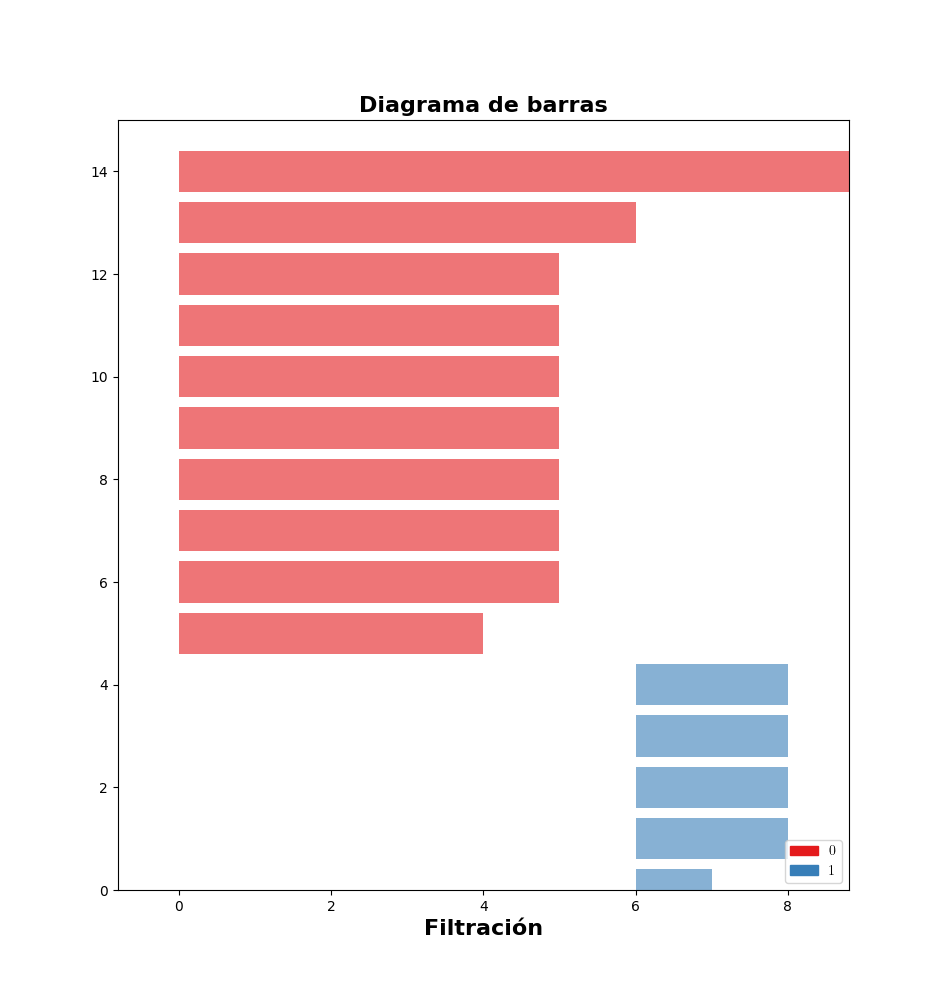
\includegraphics{Images/DiagramaBarrasEj7LOCAL.png}}
			\end{figure}
		\endminipage
		\minipage{0.5\textwidth}
			\begin{figure}[H]
				\resizebox{1.0\textwidth}{!}{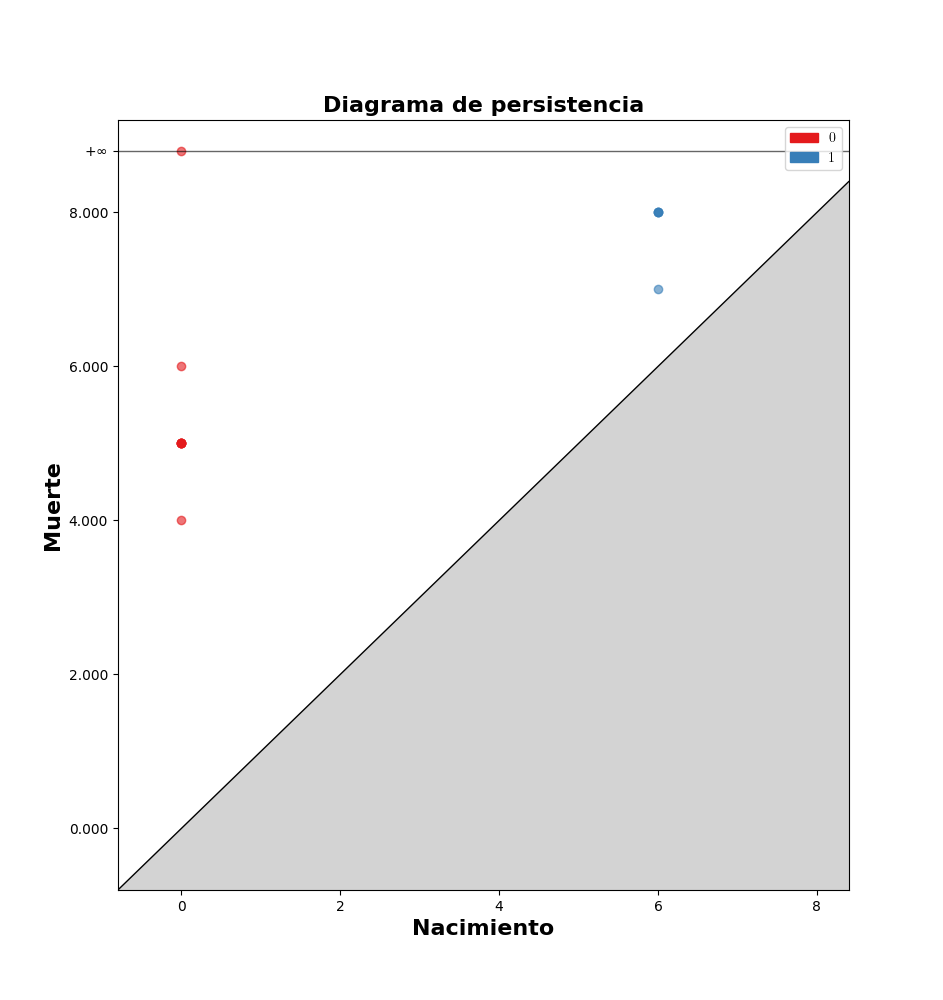
\includegraphics{Images/DiagramaPersistenciaEj7LOCAL.png}}
			\end{figure}
		\endminipage
		\caption{Diagramas de barras y persistencia asociados a la red 
		\ref{fig:ejemGlobal}}
	\end{figure}
		
		\begin{itemize}
			\item{\textbf{Interpretación global}}
		\end{itemize}
		\begin{figure}[H]
			\fbox{\minipage{0.225\textwidth}
				\begin{figure}[H]
					\resizebox{1.0\textwidth}{!}{\begin{tikzpicture}[
						roundnode/.style={circle, draw=black, thick, fill=white, minimum size=7mm},
						]
						%Nodes
						\node           (label) 	at	(1,4) 		{Filtración 0 (t=1.0)};
						\node[roundnode]      (n0) 	at 	(4,1)           {0};
						\node[roundnode]      (n1) 	at 	(4,-1)          {1};
						\node[roundnode]      (n2) 	at 	(2,2)           {2};
						\node[roundnode]      (n3) 	at 	(2,0)           {3};
						\node[roundnode]      (n4)      at 	(2,-2)		{4};
						\node[roundnode]      (n5)      at 	(0,3)		{5};
						\node[roundnode]      (n6)      at 	(0,1)		{6};
						\node[roundnode]      (n7) 	at 	(0,-1)           {7};
						\node[roundnode]      (n8) 	at 	(0,-3)           {8};
						\node[roundnode]      (n9) 	at 	(-2,2)           {9};
						\node[roundnode]      (n10) 	at 	(-2,0)           {10};
						\node[roundnode]      (n11) 	at 	(-2,-2)           {11};
						\node 		(label2) 	at 	(1,-4) 		{$\beta_{0}=10,\beta_{1}=0$};
						
						\begin{pgfonlayer}{background}
						%Lines
						\draw[thick] (n11.mid) --  (n8);
						\draw[thick] (n9.mid) --  (n5);
						\end{pgfonlayer}
					\end{tikzpicture}}	
				\end{figure}	
			\endminipage}
			\fbox{\minipage{0.225\textwidth}
				\begin{figure}[H]
					\resizebox{1.0\textwidth}{!}{\begin{tikzpicture}[
						roundnode/.style={circle, draw=black, thick, fill=white, minimum size=7mm},
						]
						%Nodes
						\node           (label) 	at	(1,4) 		{Filtración 4 (t=0.6)};
						\node[roundnode]      (n0) 	at 	(4,1)           {0};
						\node[roundnode]      (n1) 	at 	(4,-1)          {1};
						\node[roundnode]      (n2) 	at 	(2,2)           {2};
						\node[roundnode]      (n3) 	at 	(2,0)           {3};
						\node[roundnode]      (n4)      at 	(2,-2)		{4};
						\node[roundnode]      (n5)      at 	(0,3)		{5};
						\node[roundnode]      (n6)      at 	(0,1)		{6};
						\node[roundnode]      (n7) 	at 	(0,-1)           {7};
						\node[roundnode]      (n8) 	at 	(0,-3)           {8};
						\node[roundnode]      (n9) 	at 	(-2,2)           {9};
						\node[roundnode]      (n10) 	at 	(-2,0)           {10};
						\node[roundnode]      (n11) 	at 	(-2,-2)           {11};
						\node 		(label2) 	at 	(1,-4) 		{$\beta_{0}=9,\beta_{1}=0$};
						
						\begin{pgfonlayer}{background}
						%Lines
						\draw[thick] (n11.mid) --  (n8);
						\draw[thick] (n9.mid) --  (n5);
						\draw[thick] (n6.mid) --  (n2);
						\end{pgfonlayer}
					\end{tikzpicture}}	
				\end{figure}	
			\endminipage}
			\fbox{\minipage{0.225\textwidth}
				\begin{figure}[H]
					\resizebox{1.0\textwidth}{!}{\begin{tikzpicture}[
						roundnode/.style={circle, draw=black, thick, fill=white, minimum size=7mm},
						]
						%Nodes
						\node           (label) 	at	(1,4) 		{Filtración 5 (t=0.5)};
						\node[roundnode]      (n0) 	at 	(4,1)           {0};
						\node[roundnode]      (n1) 	at 	(4,-1)          {1};
						\node[roundnode]      (n2) 	at 	(2,2)           {2};
						\node[roundnode]      (n3) 	at 	(2,0)           {3};
						\node[roundnode]      (n4)      at 	(2,-2)		{4};
						\node[roundnode]      (n5)      at 	(0,3)		{5};
						\node[roundnode]      (n6)      at 	(0,1)		{6};
						\node[roundnode]      (n7) 	at 	(0,-1)           {7};
						\node[roundnode]      (n8) 	at 	(0,-3)           {8};
						\node[roundnode]      (n9) 	at 	(-2,2)           {9};
						\node[roundnode]      (n10) 	at 	(-2,0)           {10};
						\node[roundnode]      (n11) 	at 	(-2,-2)           {11};
						\node 		(label2) 	at 	(1,-4) 		{$\beta_{0}=2,\beta_{1}=0$};
						
						\begin{pgfonlayer}{background}
						%Lines
						\draw[thick] (n11.mid) --  (n8);
						\draw[thick] (n9.mid) --  (n5);
						\draw[thick] (n6.mid) --  (n2);
						\draw[thick] (n10.mid) --  (n7);
						\draw[thick] (n10.mid) --  (n6);
						\draw[thick] (n9.mid) --  (n6);
						\draw[thick] (n7.mid) --  (n4);
						\draw[thick] (n6.mid) --  (n3);
						\draw[thick] (n3.mid) --  (n1);
						\draw[thick] (n2.mid) --  (n0);
						\end{pgfonlayer}
					\end{tikzpicture}}	
				\end{figure}	
			\endminipage}
			\fbox{\minipage{0.225\textwidth}
				\begin{figure}[H]
					\resizebox{1.0\textwidth}{!}{\begin{tikzpicture}[
						roundnode/.style={circle, draw=black, fill=white, thick, minimum size=7mm},
						]
						%Nodes
						\node           (label) 	at	(1,4) 		{Filtración 6 (t=0.4)};
						\node[roundnode]      (n0) 	at 	(4,1)           {0};
						\node[roundnode]      (n1) 	at 	(4,-1)          {1};
						\node[roundnode]      (n2) 	at 	(2,2)           {2};
						\node[roundnode]      (n3) 	at 	(2,0)           {3};
						\node[roundnode]      (n4)      at 	(2,-2)		{4};
						\node[roundnode]      (n5)      at 	(0,3)		{5};
						\node[roundnode]      (n6)      at 	(0,1)		{6};
						\node[roundnode]      (n7) 	at 	(0,-1)           {7};
						\node[roundnode]      (n8) 	at 	(0,-3)           {8};
						\node[roundnode]      (n9) 	at 	(-2,2)           {9};
						\node[roundnode]      (n10) 	at 	(-2,0)           {10};
						\node[roundnode]      (n11) 	at 	(-2,-2)           {11};
						\node 		(label2) 	at 	(1,-4) 		{$\beta_{0}=1,\beta_{1}=3$};
						
						\begin{pgfonlayer}{background}
					
						\fill[fill=black!20,opacity=1] (n11.mid) -- (n8.mid) -- (n4.mid) -- cycle;
						\fill[fill=black!20,opacity=1] (n11.mid) -- (n7.mid) -- (n4.mid) -- cycle;
						\fill[fill=black!20,opacity=1] (n9.mid) -- (n6.mid) -- (n2.mid) -- cycle;
						\fill[fill=black!20,opacity=1] (n9.mid) -- (n5.mid) -- (n2.mid) -- cycle;
						
						\draw[thick] (n11.mid) --  (n8.mid);
						\draw[thick] (n11.mid) --  (n7.mid);
						\draw[thick] (n11.mid) --  (n4.mid);
						\draw[thick] (n10.mid) --  (n7.mid);
						\draw[thick] (n10.mid) --  (n6);
						\draw[thick] (n9.mid) --  (n6.mid);
						\draw[thick] (n9.mid) --  (n5.mid);
						\draw[thick] (n9.mid) --  (n2.mid);
						\draw[thick] (n8.mid) --  (n4);
						\draw[thick] (n7.mid) --  (n4);
						\draw[thick] (n7.mid) --  (n3);
						\draw[thick] (n6.mid) --  (n3);
						\draw[thick] (n6.mid) --  (n2);
						\draw[thick] (n5.mid) --  (n2);
						\draw[thick] (n4.mid) --  (n1);
						\draw[thick] (n3.mid) --  (n1);
						\draw[thick] (n3.mid) --  (n0);
						\draw[thick] (n2.mid) --  (n0);
						
						\end{pgfonlayer}
					\end{tikzpicture}}	
				\end{figure}	
			\endminipage}
		\end{figure}
		\begin{figure}[H]
			\fbox{\minipage{0.225\textwidth}
				\begin{figure}[H]
					\resizebox{1.0\textwidth}{!}{\begin{tikzpicture}[
						roundnode/.style={circle, draw=black, thick, fill=white, minimum size=7mm},
						]
						%Nodes
						\node           (label) 	at	(1,4) 		{Filtración 7 (t=0.3)};
						\node[roundnode]      (n0) 	at 	(4,1)           {0};
						\node[roundnode]      (n1) 	at 	(4,-1)          {1};
						\node[roundnode]      (n2) 	at 	(2,2)           {2};
						\node[roundnode]      (n3) 	at 	(2,0)           {3};
						\node[roundnode]      (n4)      at 	(2,-2)		{4};
						\node[roundnode]      (n5)      at 	(0,3)		{5};
						\node[roundnode]      (n6)      at 	(0,1)		{6};
						\node[roundnode]      (n7) 	at 	(0,-1)           {7};
						\node[roundnode]      (n8) 	at 	(0,-3)           {8};
						\node[roundnode]      (n9) 	at 	(-2,2)           {9};
						\node[roundnode]      (n10) 	at 	(-2,0)           {10};
						\node[roundnode]      (n11) 	at 	(-2,-2)           {11};
						\node 		(label2) 	at 	(1,-4) 		{$\beta_{0}=1,\beta_{1}=2$};
						
						\begin{pgfonlayer}{background}							
					

						\fill[fill=black!20,opacity=1] (n11.mid) -- (n8.mid) -- (n4.mid) -- cycle;
						\fill[fill=black!20,opacity=1] (n11.mid) -- (n7.mid) -- (n4.mid) -- cycle;
						\fill[fill=black!20,opacity=1] (n10.mid) to[bend right] (n4.mid) -- (n7.mid) -- cycle;
						\fill[fill=black!20,opacity=1] (n10.mid) to[bend left] (n2.mid) -- (n6.mid) -- cycle;
						\fill[fill=black!20,opacity=1] (n9.mid) -- (n6.mid) -- (n2.mid) -- cycle;
						\fill[fill=black!20,opacity=1] (n9.mid) -- (n5.mid) -- (n2.mid) -- cycle;
						\fill[fill=black!20,opacity=1] (n6.mid) to[bend left] (n1.mid) -- (n3.mid) -- cycle;
						\fill[fill=black!20,opacity=1] (n6.mid) -- (n3.mid) -- (n0.mid) -- cycle;
						\fill[fill=black!20,opacity=1] (n6.mid) -- (n2.mid) -- (n0.mid) -- cycle;
						
						\draw[thick] (n11.mid) --  (n8);
						\draw[thick] (n11.mid) --  (n7);
						\draw[thick] (n11.mid) --  (n4.mid);
						\draw[thick] (n10.mid) --  (n7);
						\draw[thick] (n10.mid) --  (n6);
						\draw[thick] (n9.mid) --  (n6);
						\draw[thick] (n9.mid) --  (n5);
						\draw[thick] (n9.mid) --  (n2.mid);
						\draw[thick] (n8.mid) --  (n4);
						\draw[thick] (n7.mid) --  (n4);
						\draw[thick] (n7.mid) --  (n3);
						\draw[thick] (n6.mid) --  (n3);
						\draw[thick] (n6.mid) --  (n2);
						\draw[thick] (n6.mid) --  (n0);
						\draw[thick] (n5.mid) --  (n2);
						\draw[thick] (n4.mid) --  (n1);
						\draw[thick] (n3.mid) --  (n1);
						\draw[thick] (n3.mid) --  (n0);
						\draw[thick] (n2.mid) --  (n0);
						\end{pgfonlayer}
					\end{tikzpicture}}	
				\end{figure}	
			\endminipage}
			\fbox{\minipage{0.225\textwidth}
				\begin{figure}[H]
					\resizebox{1.0\textwidth}{!}{\begin{tikzpicture}[
						roundnode/.style={circle, draw=black, thick, fill=white, minimum size=7mm},
						]
						%Nodes
						\node           (label) 	at	(1,4) 		{Filtración 8 (t=0.2)};
						\node[roundnode]      (n0) 	at 	(4,1)           {0};
						\node[roundnode]      (n1) 	at 	(4,-1)          {1};
						\node[roundnode]      (n2) 	at 	(2,2)           {2};
						\node[roundnode]      (n3) 	at 	(2,0)           {3};
						\node[roundnode]      (n4)      at 	(2,-2)		{4};
						\node[roundnode]      (n5)      at 	(0,3)		{5};
						\node[roundnode]      (n6)      at 	(0,1)		{6};
						\node[roundnode]      (n7) 	at 	(0,-1)           {7};
						\node[roundnode]      (n8) 	at 	(0,-3)           {8};
						\node[roundnode]      (n9) 	at 	(-2,2)           {9};
						\node[roundnode]      (n10) 	at 	(-2,0)           {10};
						\node[roundnode]      (n11) 	at 	(-2,-2)           {11};
						\node 		(label2) 	at 	(1,-4) 		{$\beta_{0}=1,\beta_{1}=0$};
						
						\begin{pgfonlayer}{background}							
					

						\fill[fill=black!20,opacity=1] (n11.mid) -- (n8.mid) -- (n4.mid) -- cycle;
						\fill[fill=black!20,opacity=1] (n11.mid) -- (n7.mid) -- (n4.mid) -- cycle;
						\fill[fill=black!20,opacity=1] (n10.mid) to[bend right] (n4.mid) -- (n7.mid) -- cycle;
						\fill[fill=black!20,opacity=1] (n10.mid) -- (n7.mid) -- (n3.mid) -- cycle;
						\fill[fill=black!20,opacity=1] (n10.mid) -- (n6.mid) -- (n3.mid) -- cycle;
						\fill[fill=black!20,opacity=1] (n10.mid) to[bend left] (n2.mid) -- (n6.mid) -- cycle;
						\fill[fill=black!20,opacity=1] (n9.mid) to[bend right] (n3.mid) -- (n6.mid) -- cycle;
						\fill[fill=black!20,opacity=1] (n9.mid) -- (n6.mid) -- (n2.mid) -- cycle;
						\fill[fill=black!20,opacity=1] (n9.mid) -- (n5.mid) -- (n2.mid) -- cycle;
						\fill[fill=black!20,opacity=1] (n7.mid) -- (n4.mid) -- (n1.mid) -- cycle;
						\fill[fill=black!20,opacity=1] (n7.mid) -- (n3.mid) -- (n1.mid) -- cycle;
						\fill[fill=black!20,opacity=1] (n6.mid) to[bend left] (n1.mid) -- (n3.mid) -- cycle;
						\fill[fill=black!20,opacity=1] (n6.mid) -- (n3.mid) -- (n0.mid) -- cycle;
						\fill[fill=black!20,opacity=1] (n6.mid) -- (n2.mid) -- (n0.mid) -- cycle;
						\fill[fill=black!20,opacity=1] (n5.mid) to[bend left] (n0.mid) -- (n2.mid) -- cycle;
						
						\draw[thick] (n11.mid) --  (n8.mid);
						\draw[thick] (n11.mid) --  (n7.mid);
						\draw[thick] (n11.mid) --  (n4.mid);
						\draw[thick] (n10.mid) --  (n7.mid);
						\draw[thick] (n10.mid) --  (n6.mid);
						\draw[thick] (n10.mid) --  (n3.mid);
						\draw[thick] (n9.mid) --  (n6.mid);
						\draw[thick] (n9.mid) --  (n5.mid);
						\draw[thick] (n9.mid) --  (n2.mid);
						\draw[thick] (n8.mid) --  (n4.mid);
						\draw[thick] (n7.mid) --  (n4.mid);
						\draw[thick] (n7.mid) --  (n3.mid);
						\draw[thick] (n7.mid) --  (n1.mid);
						\draw[thick] (n6.mid) --  (n3.mid);
						\draw[thick] (n6.mid) --  (n2.mid);
						\draw[thick] (n6.mid) --  (n0.mid);
						\draw[thick] (n5.mid) --  (n2.mid);
						\draw[thick] (n4.mid) --  (n1.mid);
						\draw[thick] (n3.mid) --  (n1.mid);
						\draw[thick] (n3.mid) --  (n0.mid);
						\draw[thick] (n2.mid) --  (n0.mid);
						\end{pgfonlayer}
					\end{tikzpicture}}	
				\end{figure}	
			\endminipage}
			\fbox{\minipage{0.225\textwidth}
				\begin{figure}[H]
					\resizebox{1.0\textwidth}{!}{\begin{tikzpicture}[
						roundnode/.style={circle, draw=black, thick, fill=white, minimum size=7mm},
						]
						%Nodes
						\node           (label) 	at	(1,4) 		{Filtración 9 (t=0.1)};
						\node[roundnode]      (n0) 	at 	(4,1)           {0};
						\node[roundnode]      (n1) 	at 	(4,-1)          {1};
						\node[roundnode]      (n2) 	at 	(2,2)           {2};
						\node[roundnode]      (n3) 	at 	(2,0)           {3};
						\node[roundnode]      (n4)      at 	(2,-2)		{4};
						\node[roundnode]      (n5)      at 	(0,3)		{5};
						\node[roundnode]      (n6)      at 	(0,1)		{6};
						\node[roundnode]      (n7) 	at 	(0,-1)           {7};
						\node[roundnode]      (n8) 	at 	(0,-3)           {8};
						\node[roundnode]      (n9) 	at 	(-2,2)           {9};
						\node[roundnode]      (n10) 	at 	(-2,0)           {10};
						\node[roundnode]      (n11) 	at 	(-2,-2)           {11};
						\node 		(label2) 	at 	(1,-4) 		{$\beta_{0}=1,\beta_{1}=0$};
						
						\begin{pgfonlayer}{background}							
					

						\fill[fill=black!20,opacity=1] (n11.mid) -- (n8.mid) -- (n4.mid) -- cycle;
						\fill[fill=black!20,opacity=1] (n11.mid) -- (n7.mid) -- (n4.mid) -- cycle;
						\fill[fill=black!20,opacity=1] (n11.mid) to[bend left] (n3.mid) -- (n7.mid) -- cycle;
						\fill[fill=black!20,opacity=1] (n10.mid) to[bend right] (n4.mid) -- (n7.mid) -- cycle;
						\fill[fill=black!20,opacity=1] (n10.mid) -- (n7.mid) -- (n3.mid) -- cycle;
						\fill[fill=black!20,opacity=1] (n10.mid) -- (n6.mid) -- (n3.mid) -- cycle;
						\fill[fill=black!20,opacity=1] (n10.mid) to[bend left] (n2.mid) -- (n6.mid) -- cycle;
						\fill[fill=black!20,opacity=1] (n9.mid) to[bend right] (n3.mid) -- (n6.mid) -- cycle;
						\fill[fill=black!20,opacity=1] (n9.mid) -- (n6.mid) -- (n2.mid) -- cycle;
						\fill[fill=black!20,opacity=1] (n9.mid) -- (n5.mid) -- (n2.mid) -- cycle;
						\fill[fill=black!20,opacity=1] (n8.mid) to[bend right] (n1.mid) -- (n4.mid) -- cycle;
						\fill[fill=black!20,opacity=1] (n7.mid) -- (n4.mid) -- (n1.mid) -- cycle;
						\fill[fill=black!20,opacity=1] (n7.mid) -- (n3.mid) -- (n1.mid) -- cycle;
						\fill[fill=black!20,opacity=1] (n7.mid) to[bend right] (n0.mid) -- (n3.mid) -- cycle;
						\fill[fill=black!20,opacity=1] (n6.mid) to[bend left] (n1.mid) -- (n3.mid) -- cycle;
						\fill[fill=black!20,opacity=1] (n6.mid) -- (n3.mid) -- (n0.mid) -- cycle;
						\fill[fill=black!20,opacity=1] (n6.mid) -- (n2.mid) -- (n0.mid) -- cycle;
						\fill[fill=black!20,opacity=1] (n5.mid) to[bend left] (n0.mid) -- (n2.mid) -- cycle;
						
						\draw[thick] (n11.mid) --  (n8.mid);
						\draw[thick] (n11.mid) --  (n7.mid);
						\draw[thick] (n11.mid) --  (n4.mid);
						\draw[thick] (n10.mid) --  (n7.mid);
						\draw[thick] (n10.mid) --  (n6.mid);
						\draw[thick] (n10.mid) --  (n3.mid);
						\draw[thick] (n9.mid) --  (n6.mid);
						\draw[thick] (n9.mid) --  (n5.mid);
						\draw[thick] (n9.mid) --  (n2.mid);
						\draw[thick] (n8.mid) --  (n4.mid);
						\draw[thick] (n7.mid) --  (n4.mid);
						\draw[thick] (n7.mid) --  (n3.mid);
						\draw[thick] (n7.mid) --  (n1.mid);
						\draw[thick] (n6.mid) --  (n3.mid);
						\draw[thick] (n6.mid) --  (n2.mid);
						\draw[thick] (n6.mid) --  (n0.mid);
						\draw[thick] (n5.mid) --  (n2.mid);
						\draw[thick] (n4.mid) --  (n1.mid);
						\draw[thick] (n3.mid) --  (n1.mid);
						\draw[thick] (n3.mid) --  (n0.mid);
						\draw[thick] (n2.mid) --  (n0.mid);
						\end{pgfonlayer}
					\end{tikzpicture}}	
				\end{figure}	
			\endminipage}
			\fbox{\minipage{0.225\textwidth}
				\begin{figure}[H]
					\resizebox{1.0\textwidth}{!}{\begin{tikzpicture}[
						roundnode/.style={circle, draw=black, thick, fill=white, minimum size=7mm},
						]
						%Nodes
						\node           (label) 	at	(1,4) 		{Filtración 10 (t=0.0)};
						\node[roundnode]      (n0) 	at 	(4,1)           {0};
						\node[roundnode]      (n1) 	at 	(4,-1)          {1};
						\node[roundnode]      (n2) 	at 	(2,2)           {2};
						\node[roundnode]      (n3) 	at 	(2,0)           {3};
						\node[roundnode]      (n4)      at 	(2,-2)		{4};
						\node[roundnode]      (n5)      at 	(0,3)		{5};
						\node[roundnode]      (n6)      at 	(0,1)		{6};
						\node[roundnode]      (n7) 	at 	(0,-1)           {7};
						\node[roundnode]      (n8) 	at 	(0,-3)           {8};
						\node[roundnode]      (n9) 	at 	(-2,2)           {9};
						\node[roundnode]      (n10) 	at 	(-2,0)           {10};
						\node[roundnode]      (n11) 	at 	(-2,-2)           {11};
						\node 		(label2) 	at 	(1,-4) 		{$\beta_{0}=1,\beta_{1}=0$};
						
						\begin{pgfonlayer}{background}							
					

						\fill[fill=black!20,opacity=1] (n11.mid) -- (n8.mid) -- (n4.mid) -- cycle;
						\fill[fill=black!20,opacity=1] (n11.mid) -- (n7.mid) -- (n4.mid) -- cycle;
						\fill[fill=black!20,opacity=1] (n11.mid) to[bend left] (n3.mid) -- (n7.mid) -- cycle;
						\fill[fill=black!20,opacity=1] (n10.mid) to[bend right] (n4.mid) -- (n7.mid) -- cycle;
						\fill[fill=black!20,opacity=1] (n10.mid) -- (n7.mid) -- (n3.mid) -- cycle;
						\fill[fill=black!20,opacity=1] (n10.mid) -- (n6.mid) -- (n3.mid) -- cycle;
						\fill[fill=black!20,opacity=1] (n10.mid) to[bend left] (n2.mid) -- (n6.mid) -- cycle;
						\fill[fill=black!20,opacity=1] (n9.mid) to[bend right] (n3.mid) -- (n6.mid) -- cycle;
						\fill[fill=black!20,opacity=1] (n9.mid) -- (n6.mid) -- (n2.mid) -- cycle;
						\fill[fill=black!20,opacity=1] (n9.mid) -- (n5.mid) -- (n2.mid) -- cycle;
						\fill[fill=black!20,opacity=1] (n8.mid) to[bend right] (n1.mid) -- (n4.mid) -- cycle;
						\fill[fill=black!20,opacity=1] (n7.mid) -- (n4.mid) -- (n1.mid) -- cycle;
						\fill[fill=black!20,opacity=1] (n7.mid) -- (n3.mid) -- (n1.mid) -- cycle;
						\fill[fill=black!20,opacity=1] (n7.mid) to[bend right] (n0.mid) -- (n3.mid) -- cycle;
						\fill[fill=black!20,opacity=1] (n6.mid) to[bend left] (n1.mid) -- (n3.mid) -- cycle;
						\fill[fill=black!20,opacity=1] (n6.mid) -- (n3.mid) -- (n0.mid) -- cycle;
						\fill[fill=black!20,opacity=1] (n6.mid) -- (n2.mid) -- (n0.mid) -- cycle;
						\fill[fill=black!20,opacity=1] (n5.mid) to[bend left] (n0.mid) -- (n2.mid) -- cycle;
						
						\draw[thick] (n11.mid) --  (n8.mid);
						\draw[thick] (n11.mid) --  (n7.mid);
						\draw[thick] (n11.mid) --  (n4.mid);
						\draw[thick] (n10.mid) --  (n7.mid);
						\draw[thick] (n10.mid) --  (n6.mid);
						\draw[thick] (n10.mid) --  (n3.mid);
						\draw[thick] (n9.mid) --  (n6.mid);
						\draw[thick] (n9.mid) --  (n5.mid);
						\draw[thick] (n9.mid) --  (n2.mid);
						\draw[thick] (n8.mid) --  (n4.mid);
						\draw[thick] (n7.mid) --  (n4.mid);
						\draw[thick] (n7.mid) --  (n3.mid);
						\draw[thick] (n7.mid) --  (n1.mid);
						\draw[thick] (n6.mid) --  (n3.mid);
						\draw[thick] (n6.mid) --  (n2.mid);
						\draw[thick] (n6.mid) --  (n0.mid);
						\draw[thick] (n5.mid) --  (n2.mid);
						\draw[thick] (n4.mid) --  (n1.mid);
						\draw[thick] (n3.mid) --  (n1.mid);
						\draw[thick] (n3.mid) --  (n0.mid);
						\draw[thick] (n2.mid) --  (n0.mid);
						\end{pgfonlayer}
					\end{tikzpicture}}	
				\end{figure}	
			\endminipage}
		\end{figure}
		\begin{figure}[H]
			\minipage{0.5\textwidth}
				\begin{figure}[H]
					\resizebox{1.0\textwidth}{!}{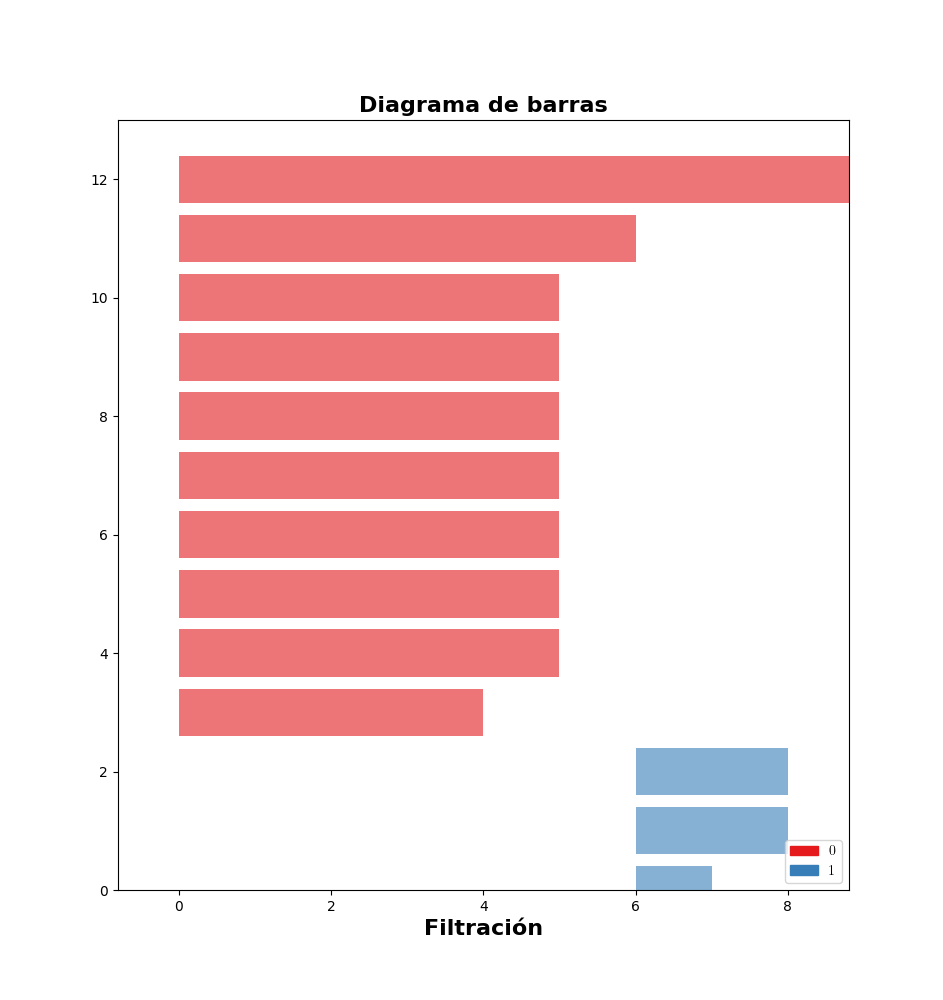
\includegraphics{Images/DiagramaBarrasEj7GLOBAL.png}}
				\end{figure}
			\endminipage
			\minipage{0.5\textwidth}
				\begin{figure}[H]
					\resizebox{1.0\textwidth}{!}{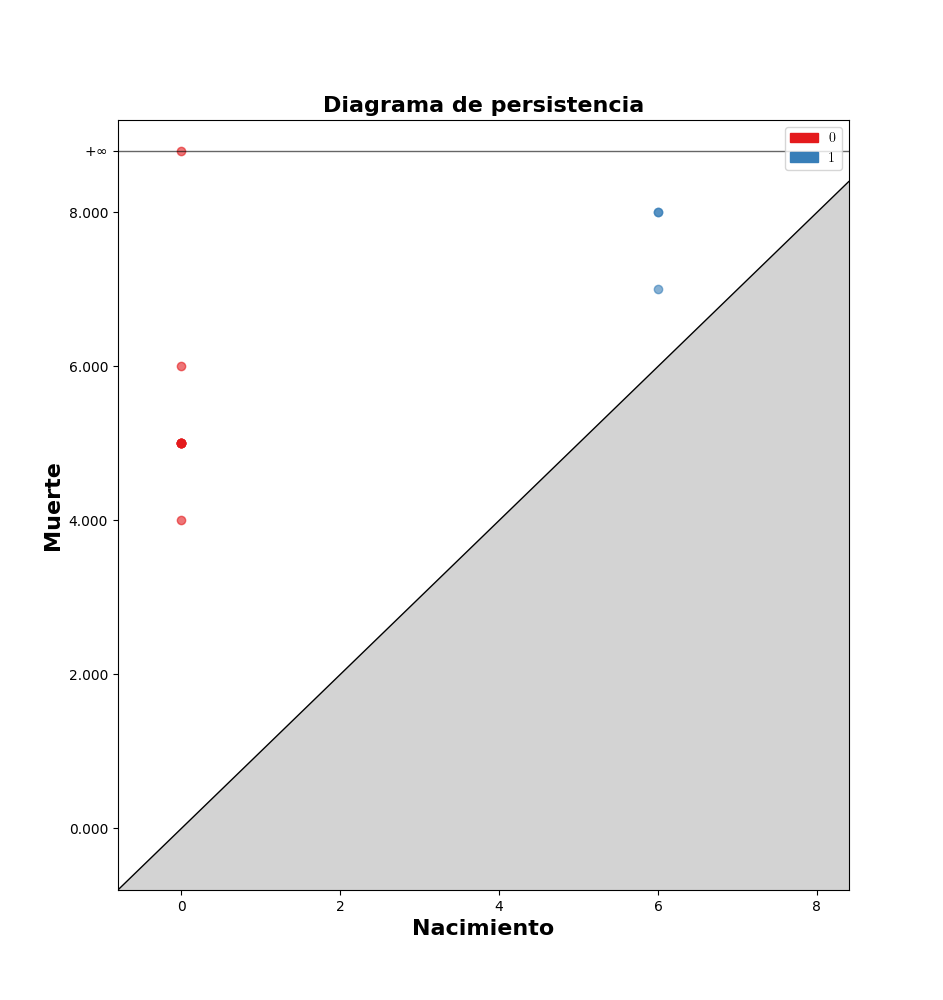
\includegraphics{Images/DiagramaPersistenciaEj7GLOBAL.png}}
				\end{figure}
			\endminipage
		\end{figure}
		\begin{remark}
			Para una mayor claridad, en los dibujos de las filtraciones se han omitido algunas aristas.
		\end{remark}
	\end{ejem}	
	Del ejemplo anterior podemos extraer unas conclusiones muy importantes. Por una parte, observamos que si las neuronas de entrada se conectan
	directamente a las de salida, el conocimiento de la red será ``pobre" ya que será equivalente a la detección de patrones. Por otra parte,
	el incremento del número de Betti $\beta_{1}$ indica que la red determina la neurona de llegada por combinación de las neuronas de salida. De este modo,
	podemos suponer que el aumento de $\beta_{1}$ releja la complejidad del conocimiento adquirido por la red. Por lo tanto, mediante el uso de la homología persistente
	seremos capaces de medir la complejidad del conocimiento adquirido por la red.


	\section{Interpretación local. Algoritmos y programas}

	\section{Ejemplos}

	\chapter{Conclusiones}

	\newpage
	\nocite{*}
	\bibliographystyle{babplain}
	\bibliography{Referencias}
\end{document} 

